% !TeX spellcheck = pl_PL-Polish

\documentclass[11pt, xcolor={dvipsnames,svgnames},aspectratio=169]{beamer}
%\hypersetup{colorlinks}
\usepackage{etex} % tikz needs it
%\usepackage[cp1250]{inputenc}
\usepackage{polski}
\usepackage[OT4]{fontenc} % doesn't change - default, and best?
%\usepackage[T1]{fontenc} % thinner, a bit more machine like
%\usepackage{times} % serif
\usepackage{amsfonts}
\usepackage{amsmath}
\usepackage{amsthm}
\usepackage{amsbsy}
\usepackage{amscd}
\usepackage{bbm}
\usepackage[mathscr]{eucal} 
%\usepackage{subfigure}
%\usepackage{ctable}
\usepackage{pifont}
\usepackage{color}
\usepackage{booktabs}
\usepackage{colortbl}
\usepackage{marvosym}
\usepackage{wasysym}
\usepackage[normalem]{ulem}
\usepackage{multicol}
\usepackage[makeroom]{cancel}
\usepackage{soul}
\definecolor{orange}{rgb}{0.75,0.33,0}
\newcommand{\myemph}[1]{\textcolor{orange}{#1}}


\usepackage{isomath}
\usepackage{soul}


%\newcommand{\source}[1]{\tiny\begin{flushright}(źródło ilustacji: \texttt{#1})\end{flushright}\normalsize}

 
\usetheme{iitisask}
\title[]{Sieć MLP -- analiza działania dla przykładowych danych}
\author{Przemysław Głomb}
\date{redaktor pomocniczy: Bartłomiej Gardas}

\theoremstyle{plain}
\newcommand{\scaly}{0.7}
\newcommand{\skippy}{\vskip 0.1cm\pause}


\newcommand{\scalethree}{0.5}
\newcommand{\scaletwo}{0.75}
 
 
\begin{document}

\frame{\maketitle}


% < = = MARK = = >   39 min  (of 180 min) | plan-2xchat-3xnnintro-środ-python-*RUN(2x)-*Task(3x)


\section{Sieci neuronowe -- ,,case study'' weryfikacji danych}


\begin{frame}
	\frametitle{Pomiar ciśnienia na wejściu do strefy wodociągowej}
	\begin{center}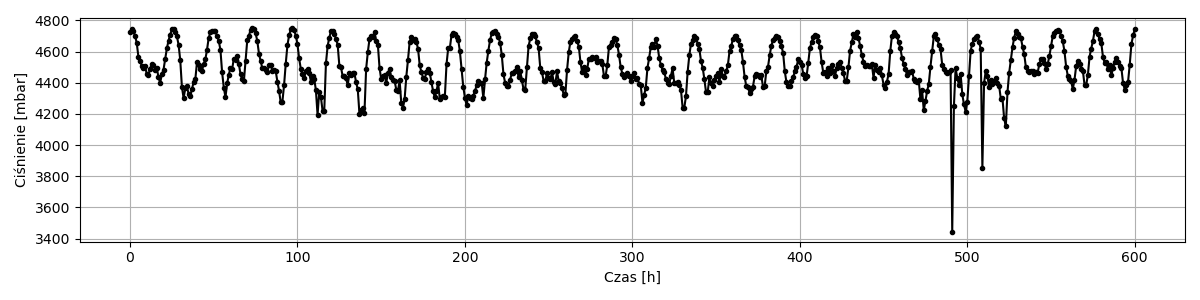
\includegraphics[width=\textwidth]{images/press1.png}\end{center}
\end{frame}
\begin{frame}
	\frametitle{Pomiar ciśnienia na wejściu do strefy wodociągowej}
	\begin{center}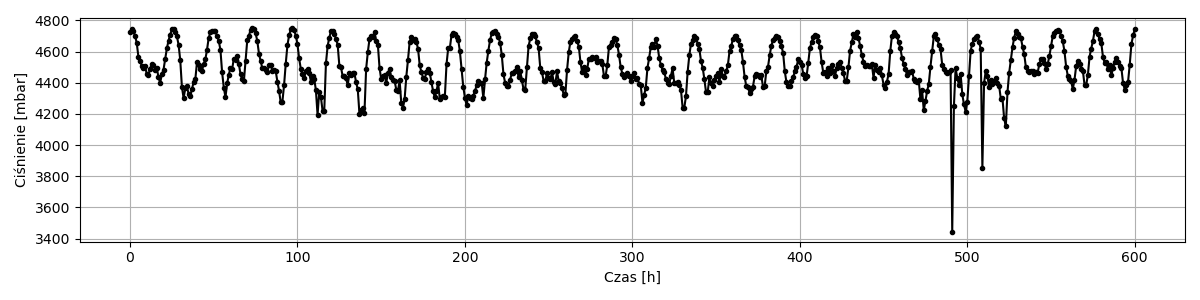
\includegraphics[width=\scalethree\textwidth]{images/press1.png}\end{center}
	\begin{center}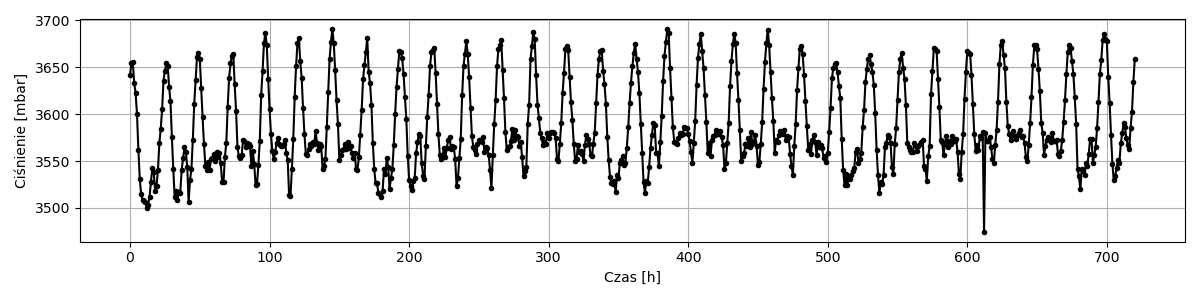
\includegraphics[width=\scalethree\textwidth]{images/press2.png}\end{center}
	\begin{center}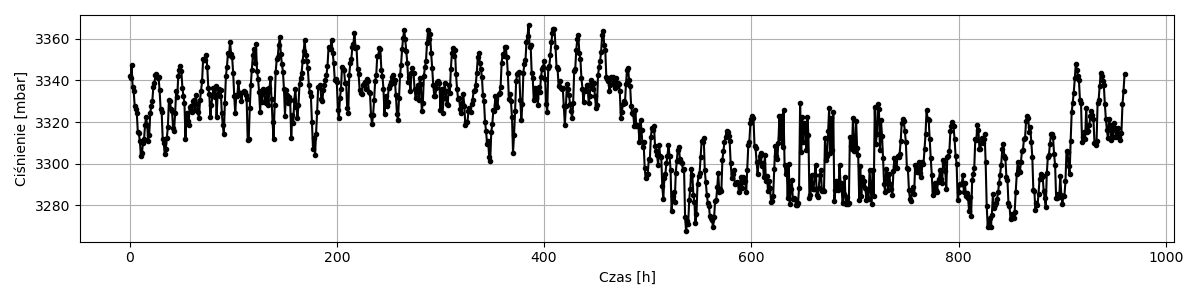
\includegraphics[width=\scalethree\textwidth]{images/press3.png}\end{center}
\end{frame}
\begin{frame}
	\frametitle{Weryfikacja danych}
	\begin{center}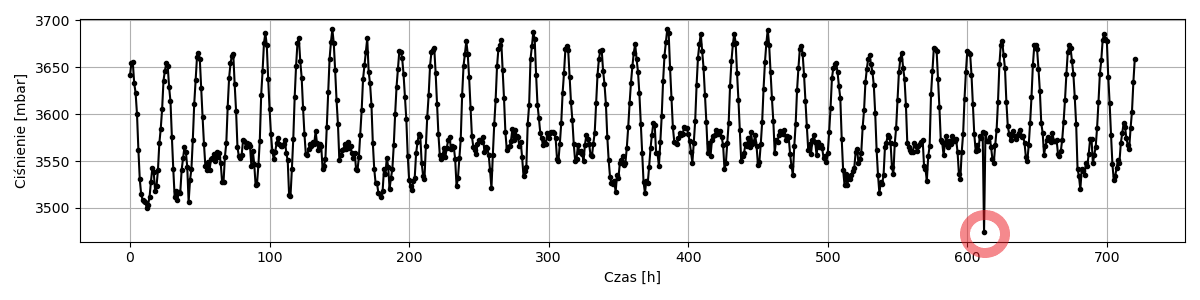
\includegraphics[width=\textwidth]{images/press2a.png}\end{center}
\end{frame}
\begin{frame}
	\frametitle{Anomalia $\rightarrow$ ,,nietypowe zachowanie''}
	\begin{center}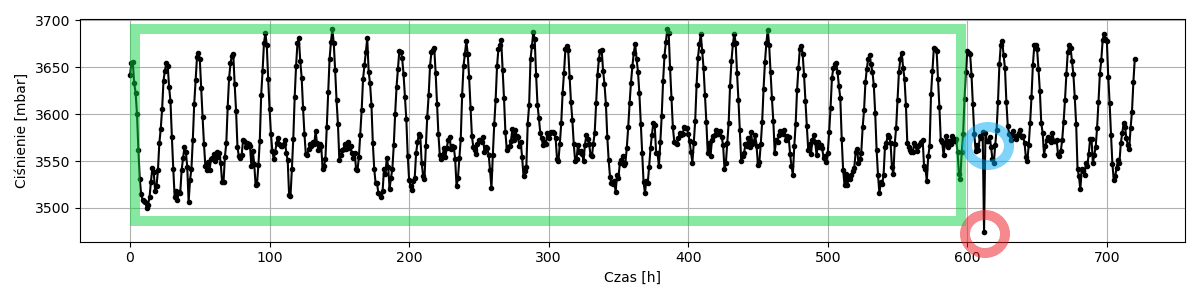
\includegraphics[width=\textwidth]{images/press2aa.png}\end{center}
\end{frame}
\begin{frame}
	\frametitle{Weryfikacja na podstawie predykcji z modelu}
	\begin{center}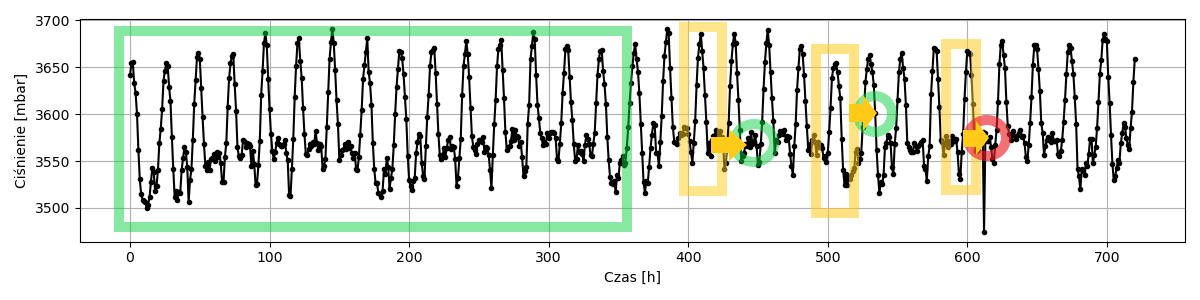
\includegraphics[width=\textwidth]{images/press2aaa.png}\end{center}
\end{frame}

%\begin{frame}
%	\texttt{ex\_nn\_demo1.py}
%	\vskip 1cm
%	\texttt{ex\_nn\_demo\_windows.py}
%\end{frame}

%\begin{frame}[fragile]
%	\frametitle{Eksperyment -- model sieci neuronowej dla predykcji}
%	\begin{verbatim}
%n_window, layers, n_training = 24, [3, 2], 400
%		
%signal = (signal - np.mean(signal)) / np.std(signal)
%X, y, _, _ = get_windows(signal, n=n_window)
%X_training, y_training = X[:n_training], y[:n_training]
%nn = MLPRegressor(hidden_layer_sizes=layers, max_iter=1000)
%nn.fit(X_training, y_training)
%yn = nn.predict(X)
%	\end{verbatim}
%\end{frame}

\begin{frame}	\frametitle{Jeden, wyjściowy neuron}
	\texttt{n\_window, layers = 1, []}
	\begin{center}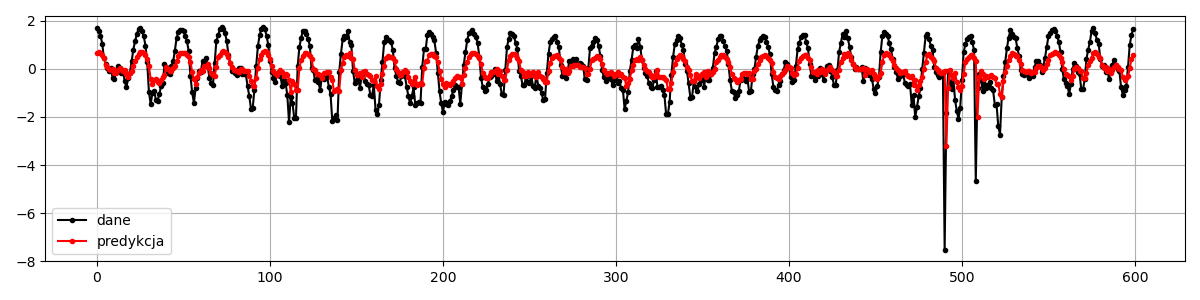
\includegraphics[width=\scaletwo\textwidth]{images/no_pred.png}\end{center}
	\begin{center}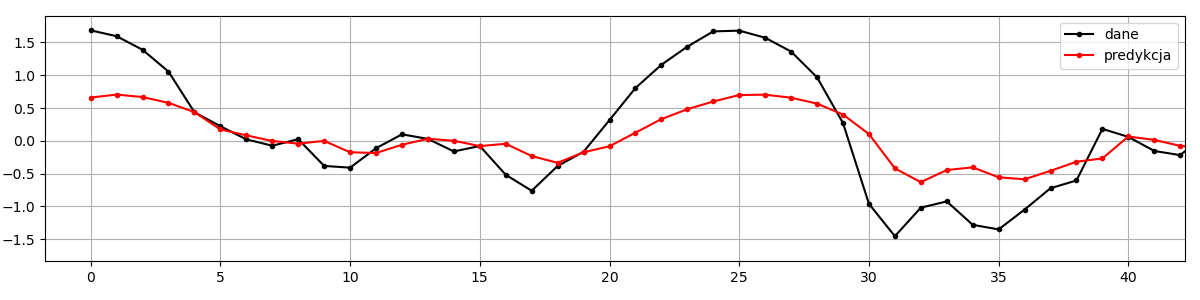
\includegraphics[width=\scaletwo\textwidth]{images/no_zoom.png}\end{center}
\end{frame}
\begin{frame}	\frametitle{Jeden, wyjściowy neuron}
	\texttt{n\_window, layers = 1, []}
	\begin{center}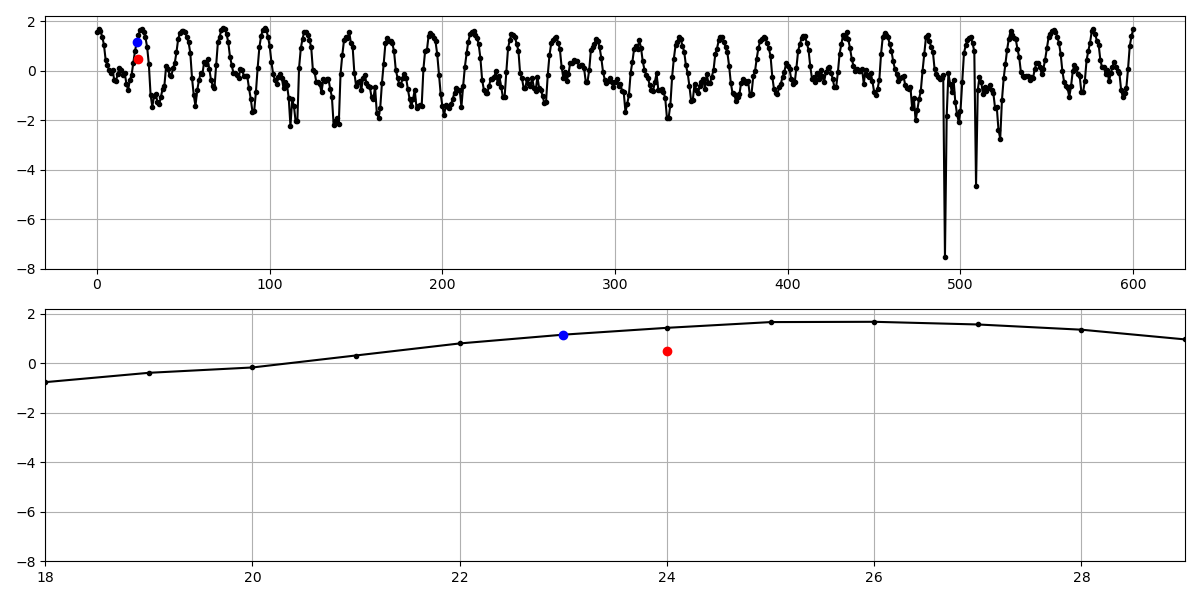
\includegraphics[width=\scaletwo\textwidth]{images/no_out.png}\end{center}
\end{frame}
\begin{frame}	\frametitle{Jeden, wyjściowy neuron}
	\texttt{n\_window, layers = 1, []}
	\begin{center}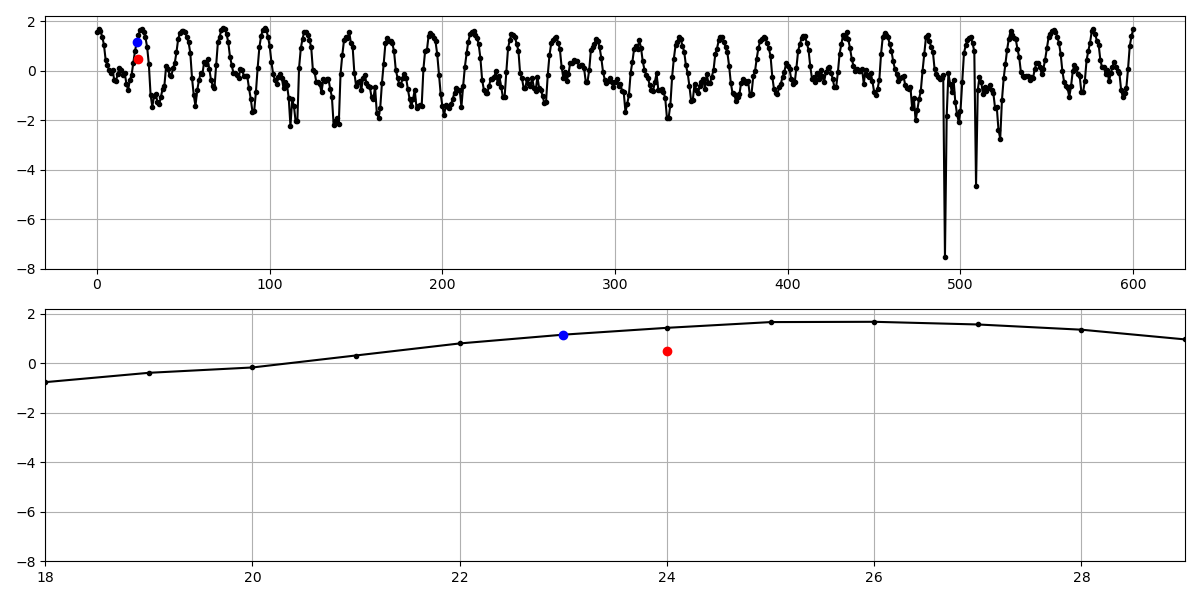
\includegraphics[width=0.49\textwidth]{images/no_out.png}
		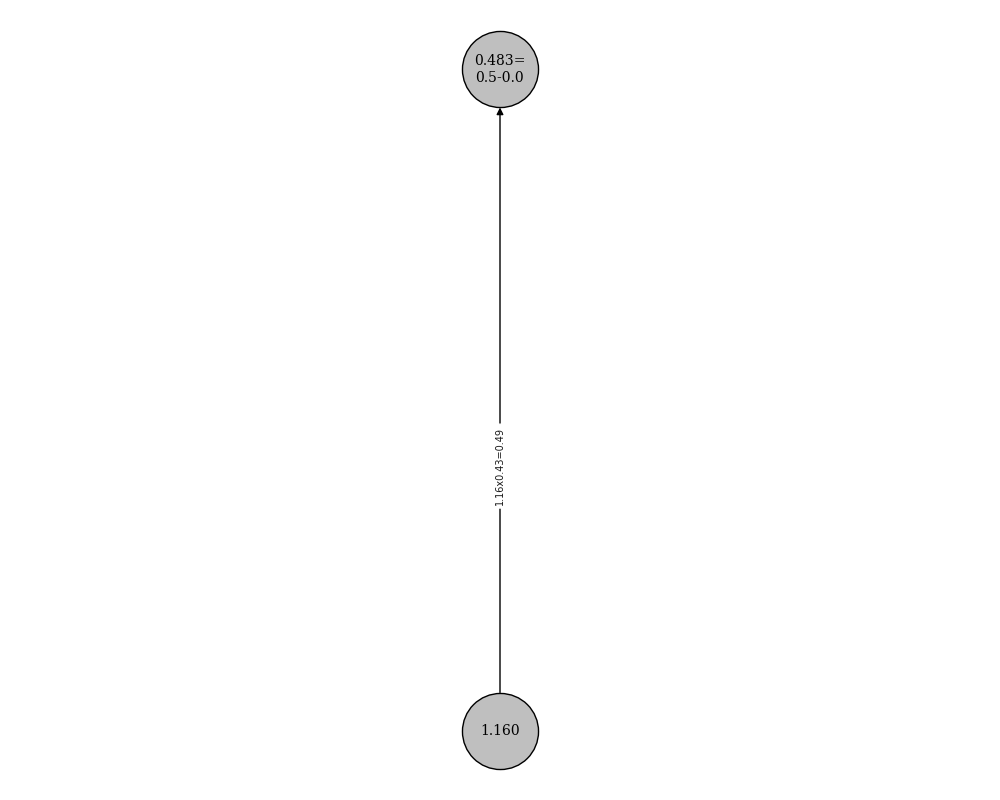
\includegraphics[width=0.49\textwidth]{images/no_in.png}\end{center}
\end{frame}

\begin{frame}	\frametitle{Jeden neuron w warstwie ukrytej}
	\texttt{n\_window, layers = 1, [1]}
	\begin{center}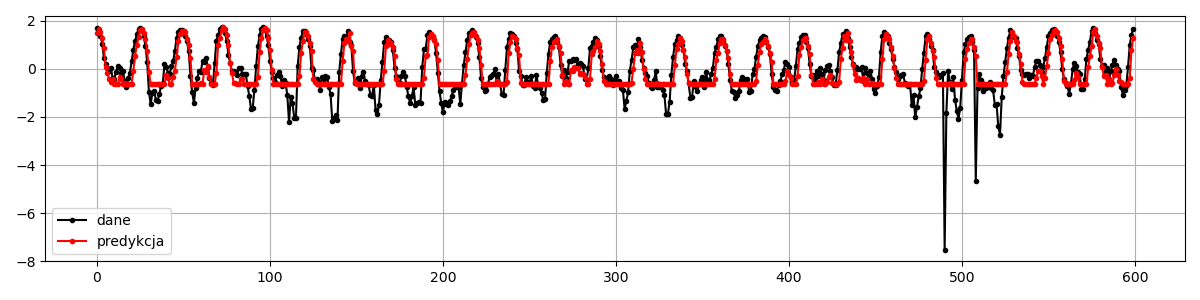
\includegraphics[width=\textwidth]{images/one_pred.png}\end{center}
\end{frame}
\begin{frame}	\frametitle{Jeden neuron w warstwie ukrytej}
	\texttt{n\_window, layers = 1, [1]}
	\begin{center}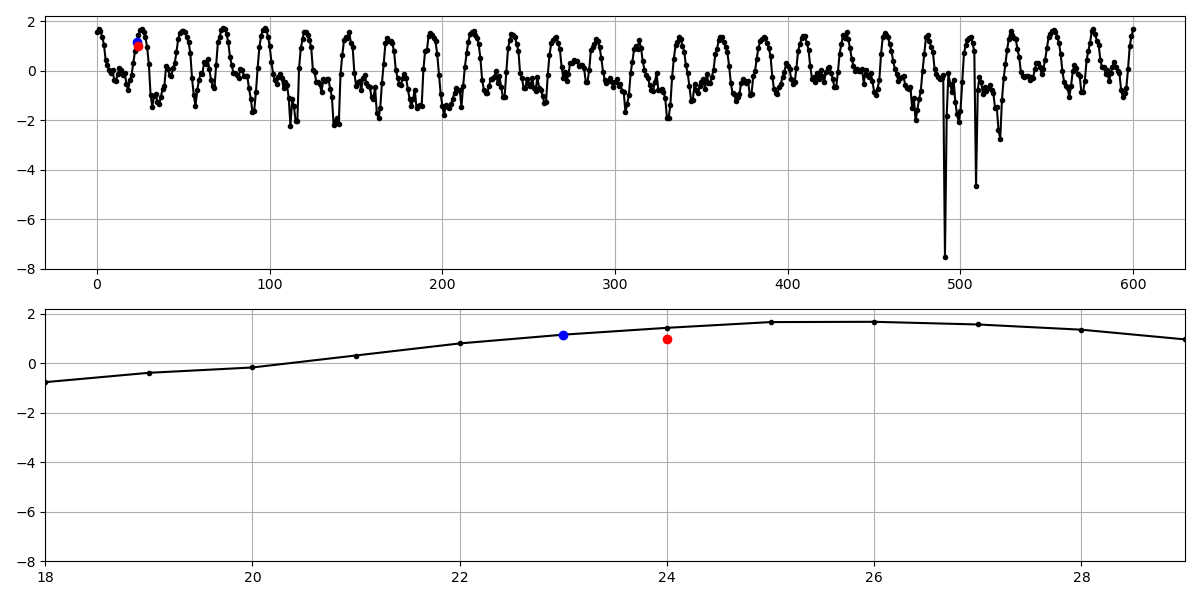
\includegraphics[width=\scaletwo\textwidth]{images/one_out.png}\end{center}
\end{frame}
\begin{frame}	\frametitle{Jeden neuron w warstwie ukrytej}
	\texttt{n\_window, layers = 1, [1]}
	\begin{center}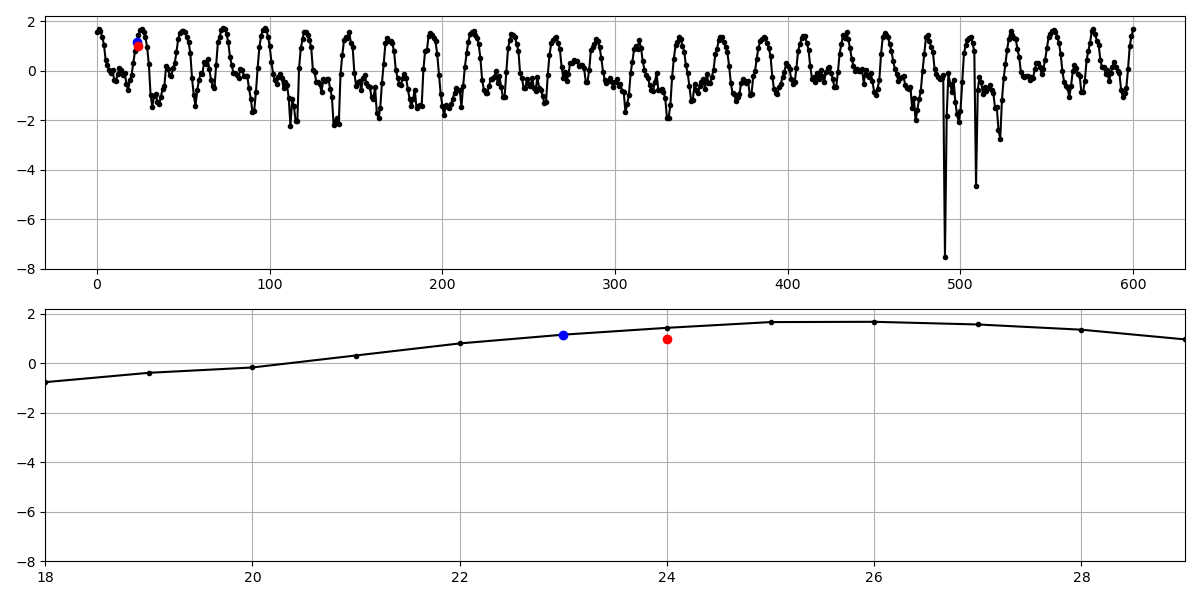
\includegraphics[width=0.49\textwidth]{images/one_out.png}
		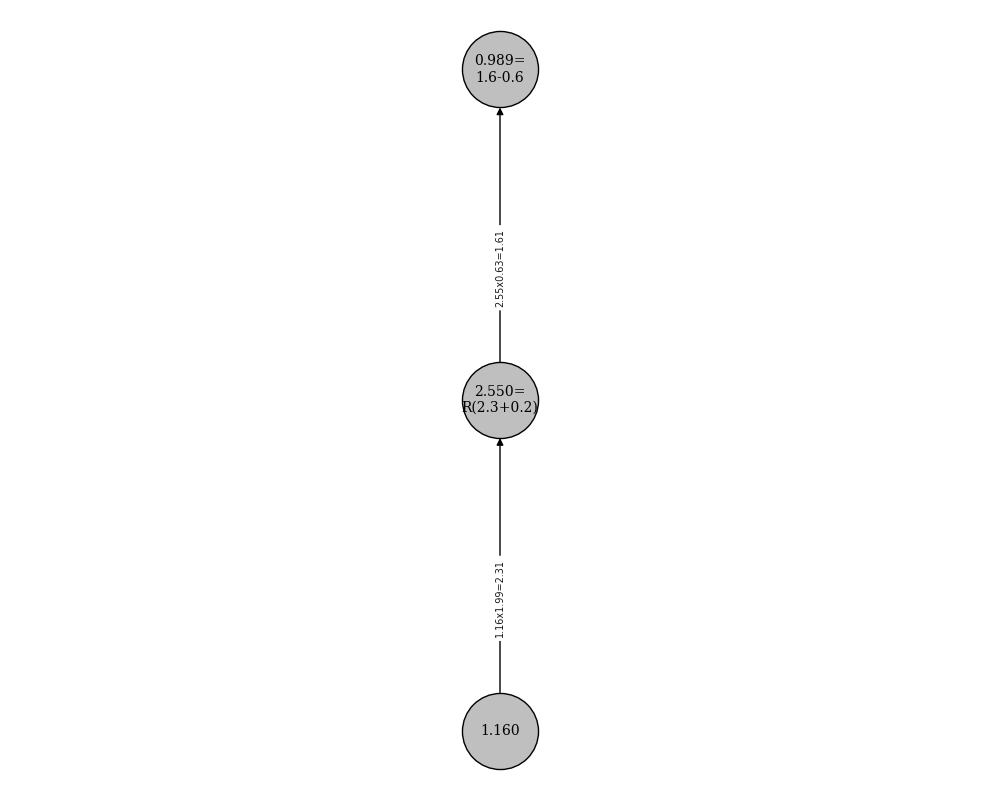
\includegraphics[width=0.49\textwidth]{images/one_in.png}\end{center}
\end{frame}

\begin{frame}	\frametitle{Dwa pomiary w historii}
	\texttt{n\_window, layers = 2, [1]}
	\begin{center}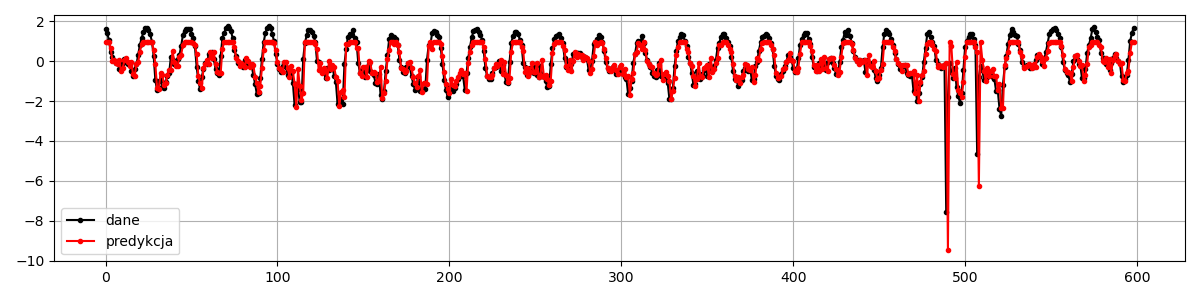
\includegraphics[width=\textwidth]{images/oneh2_pred.png}\end{center}
\end{frame}
\begin{frame}	\frametitle{Dwa pomiary w historii}
	\texttt{n\_window, layers = 2, [1]}
	\begin{center}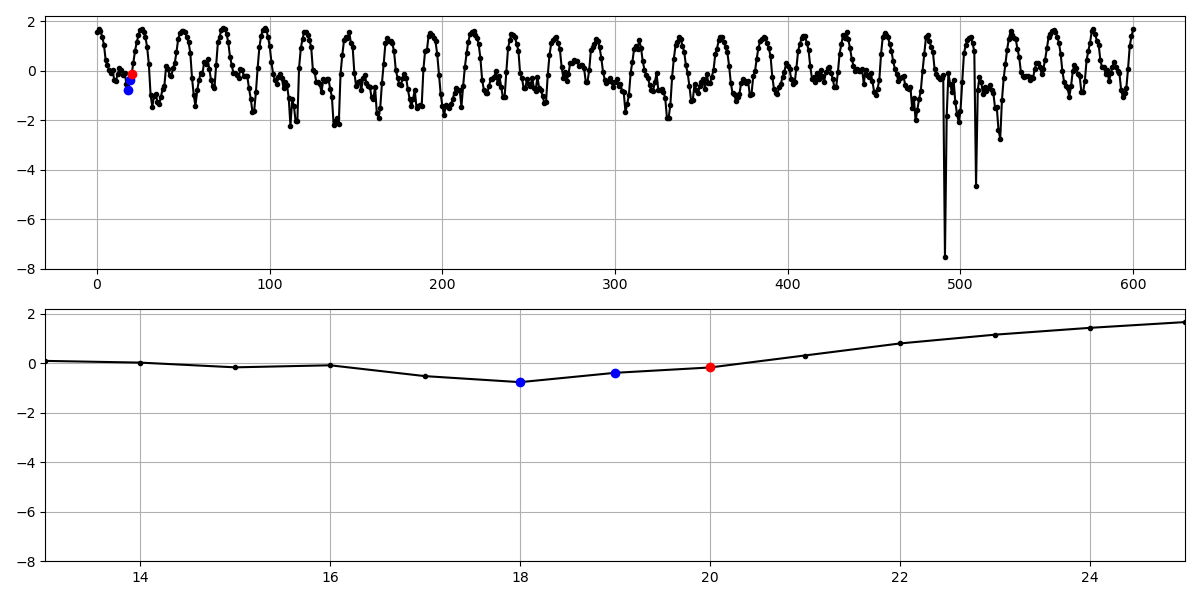
\includegraphics[width=\scaletwo\textwidth]{images/oneh2_out.png}\end{center}
\end{frame}
\begin{frame}	\frametitle{Dwa pomiary w historii}
	\texttt{n\_window, layers = 2, [1]}
	\begin{center}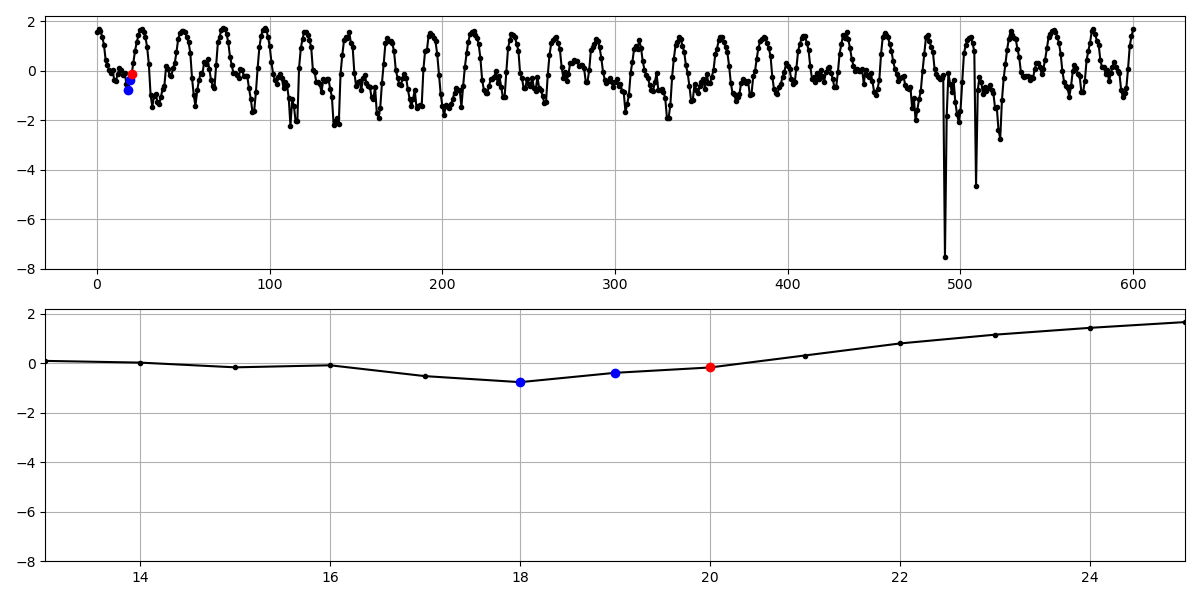
\includegraphics[width=0.49\textwidth]{images/oneh2_out.png}
		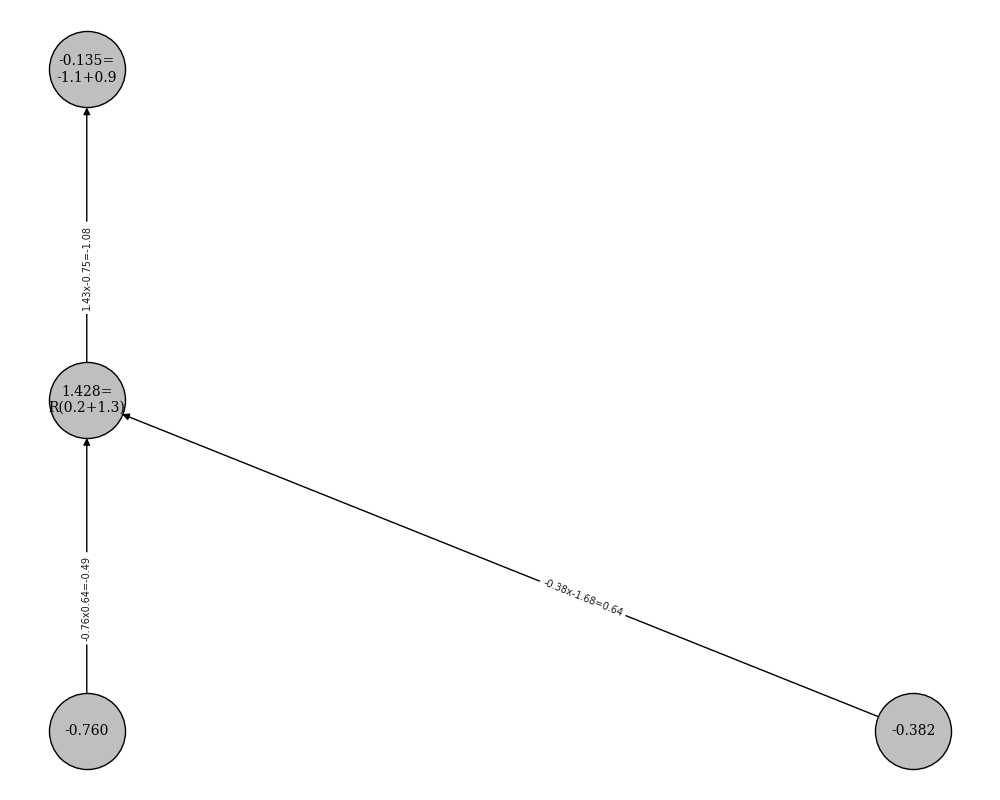
\includegraphics[width=0.49\textwidth]{images/oneh2_in.png}\end{center}
\end{frame}

\begin{frame}	\frametitle{2 pomiary w historii i 2 neurony w w. ukrytej}
	\texttt{n\_window, layers = 2, [2]}
	\begin{center}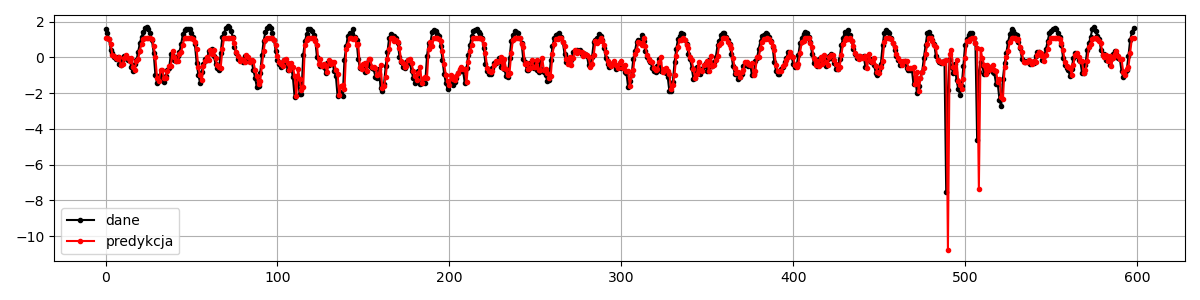
\includegraphics[width=\textwidth]{images/twoh2_pred.png}\end{center}
\end{frame}
\begin{frame}	\frametitle{2 pomiary w historii i 2 neurony w w. ukrytej}
	\texttt{n\_window, layers = 2, [2]}
	\begin{center}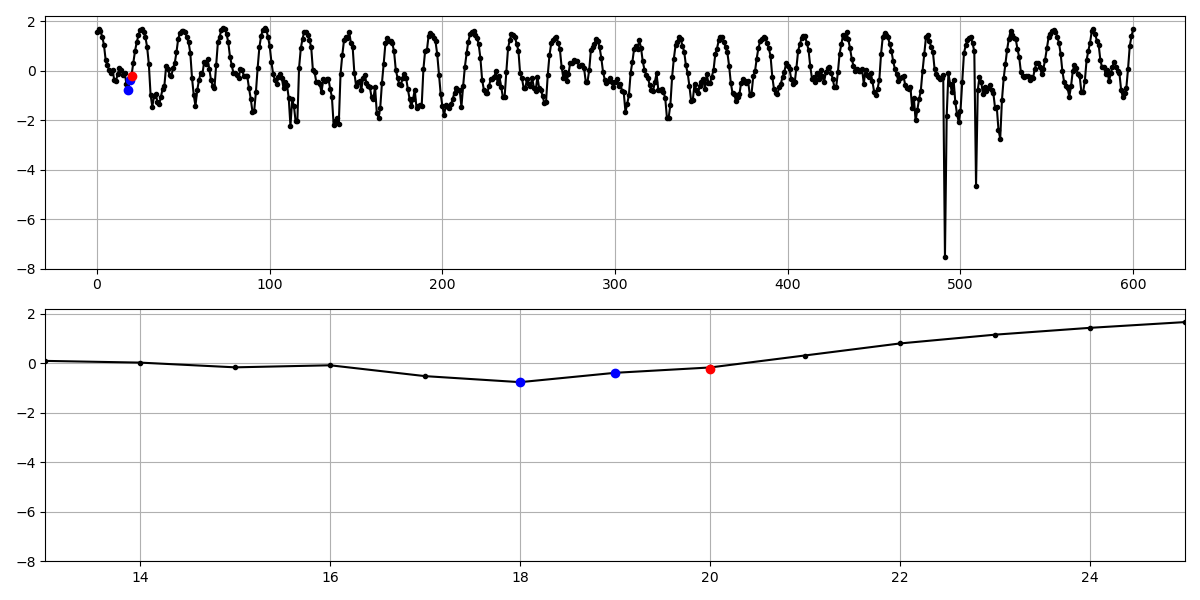
\includegraphics[width=\scaletwo\textwidth]{images/twoh2_out.png}\end{center}
\end{frame}
\begin{frame}	\frametitle{2 pomiary w historii i 2 neurony w w. ukrytej}
	\texttt{n\_window, layers = 2, [2]}
	\begin{center}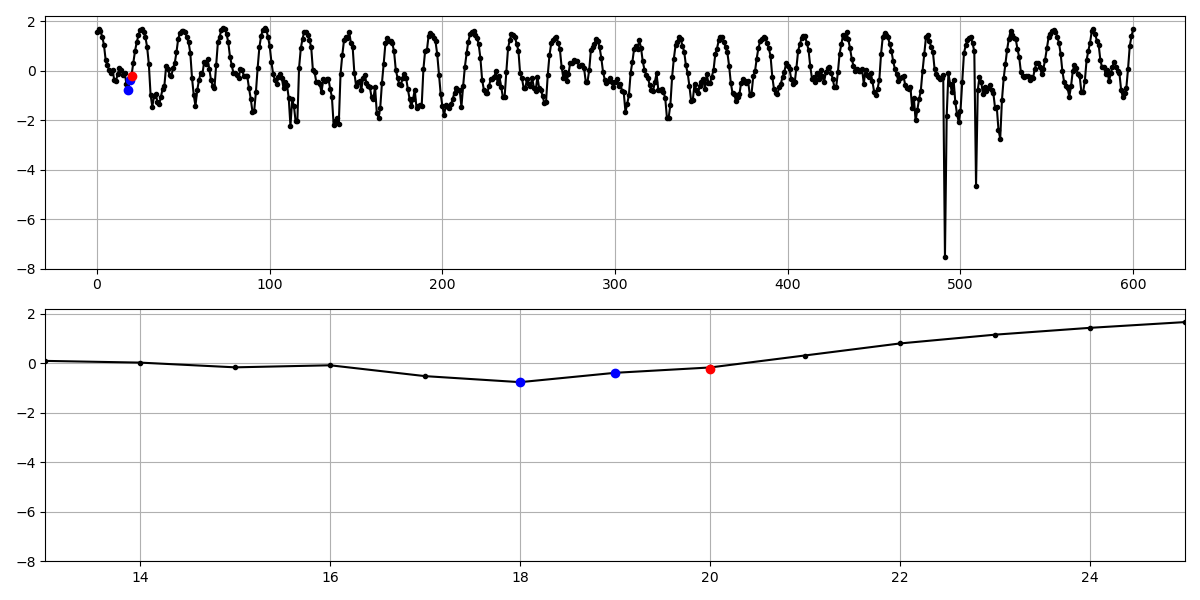
\includegraphics[width=0.49\textwidth]{images/twoh2_out.png}
		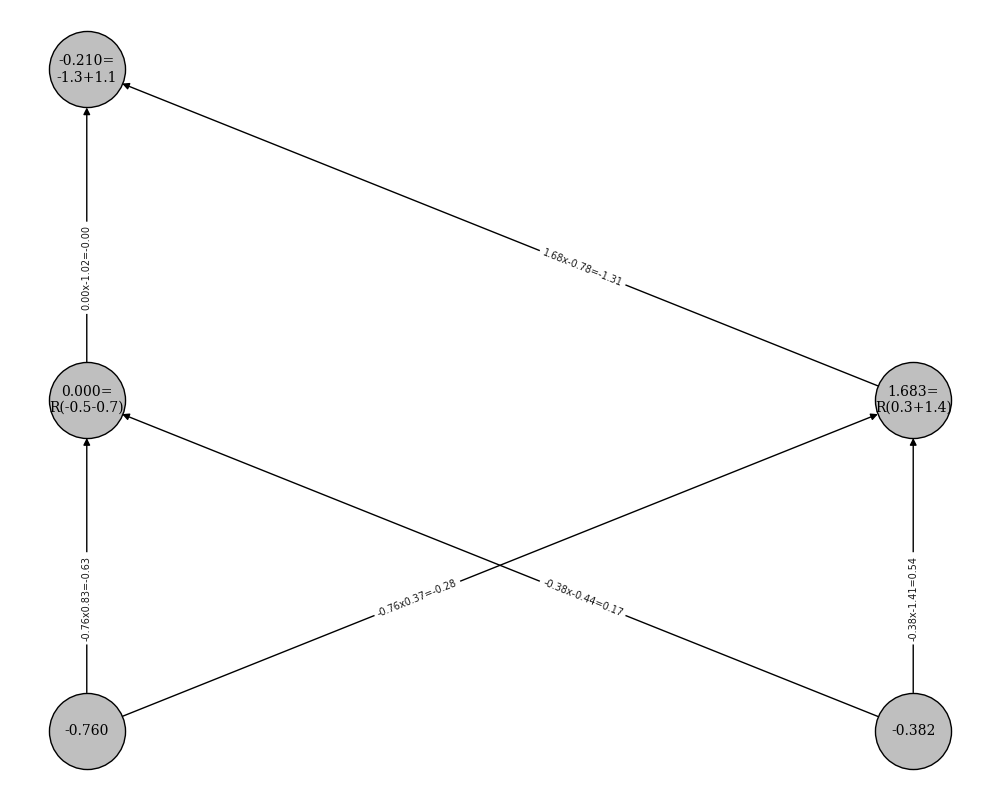
\includegraphics[width=0.49\textwidth]{images/twoh2_in.png}\end{center}
\end{frame}

\begin{frame}	\frametitle{10 pomiarów w historii i 2 neurony w w. ukrytej}
	\texttt{n\_window, layers = 10, [2]}
	\begin{center}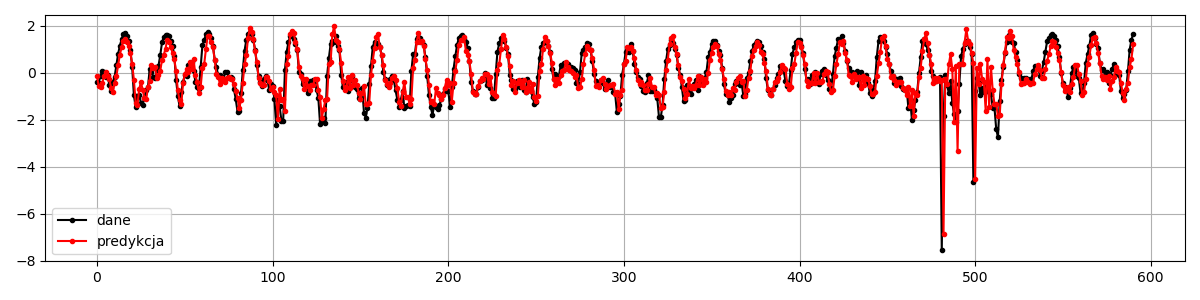
\includegraphics[width=\scaletwo\textwidth]{images/twohm_pred.png}\end{center}
	\begin{center}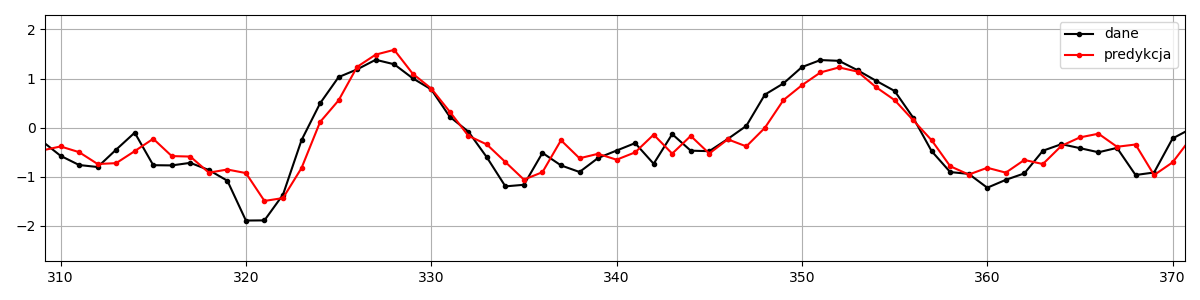
\includegraphics[width=\scaletwo\textwidth]{images/twohm_zoom.png}\end{center}
\end{frame}
\begin{frame}	\frametitle{10 pomiarów w historii i 2 neurony w w. ukrytej}
	\texttt{n\_window, layers = 10, [2]}
	\begin{center}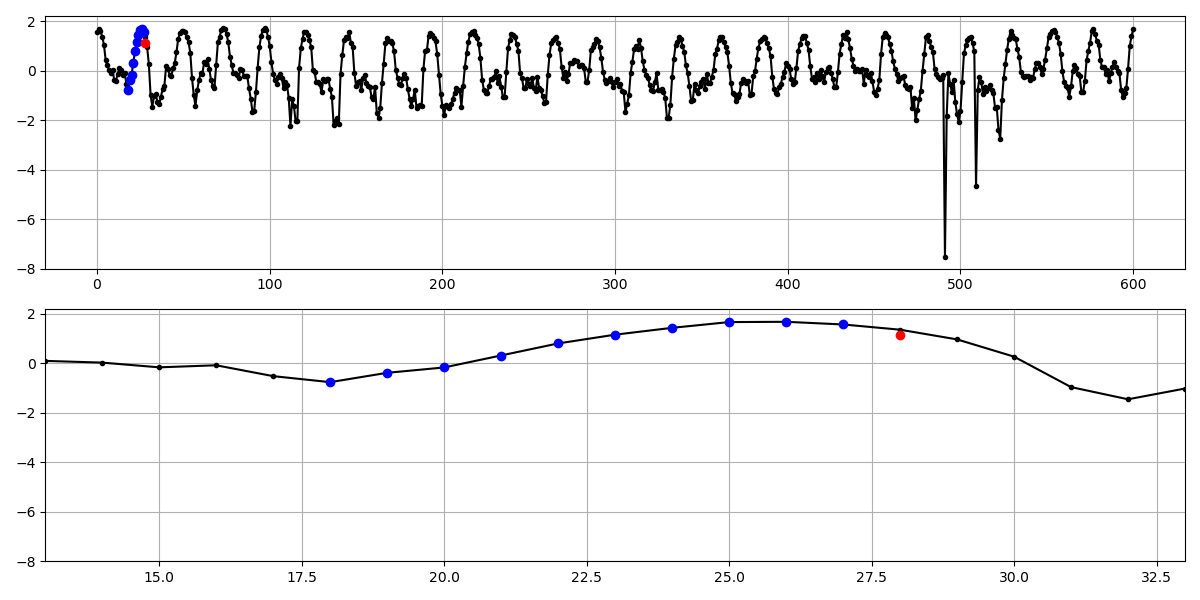
\includegraphics[width=\scaletwo\textwidth]{images/twohm_out.png}\end{center}
\end{frame}
\begin{frame}	\frametitle{10 pomiarów w historii i 2 neurony w w. ukrytej}
	\texttt{n\_window, layers = 10, [2]}
	\begin{center}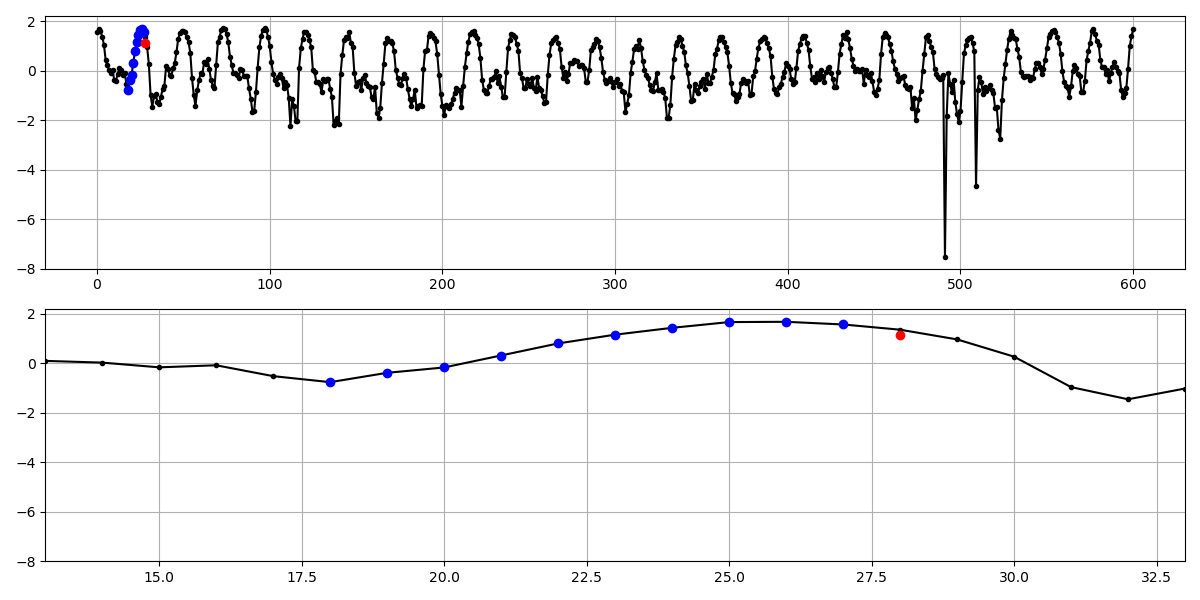
\includegraphics[width=0.49\textwidth]{images/twohm_out.png}
		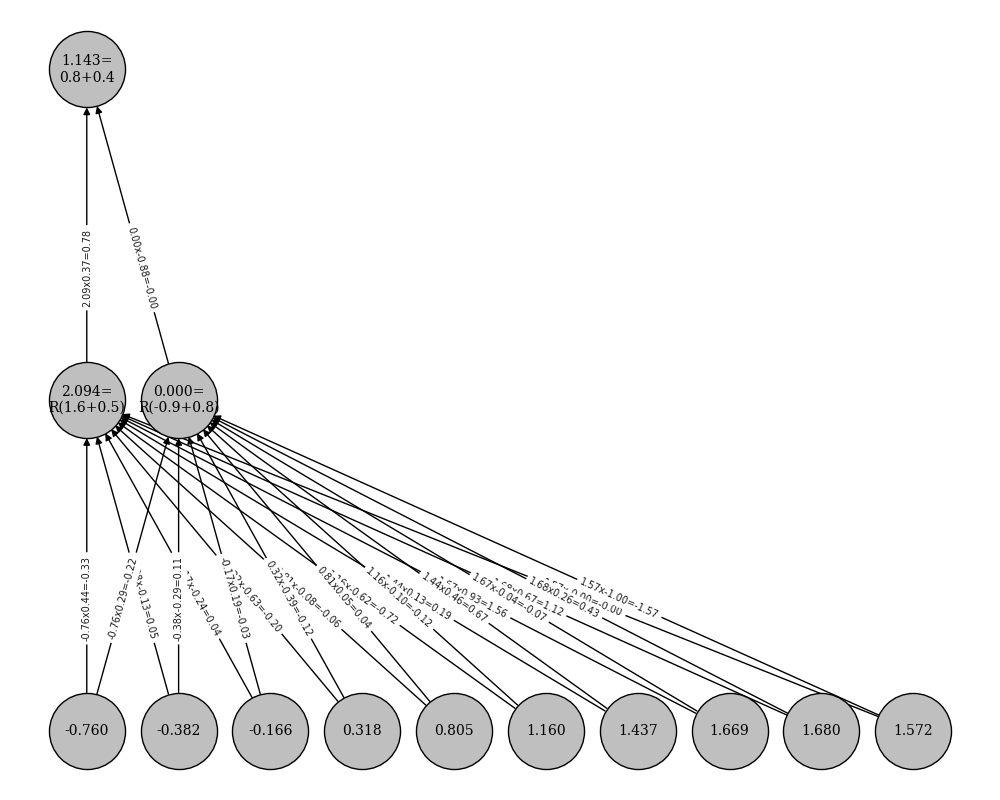
\includegraphics[width=0.49\textwidth]{images/twohm_in.png}\end{center}
\end{frame}

\begin{frame}	\frametitle{10 pomiarów w historii i 3 neurony w w. ukrytej}
	\texttt{n\_window, layers = 10, [3]}
	\begin{center}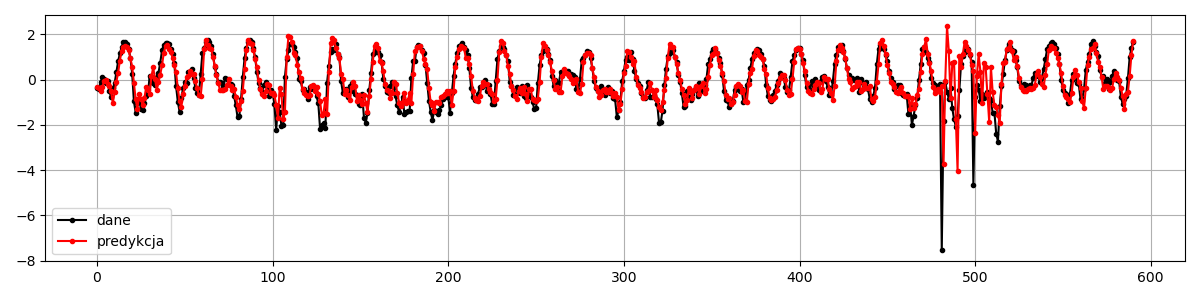
\includegraphics[width=\scaletwo\textwidth]{images/threehm_pred.png}\end{center}
	\begin{center}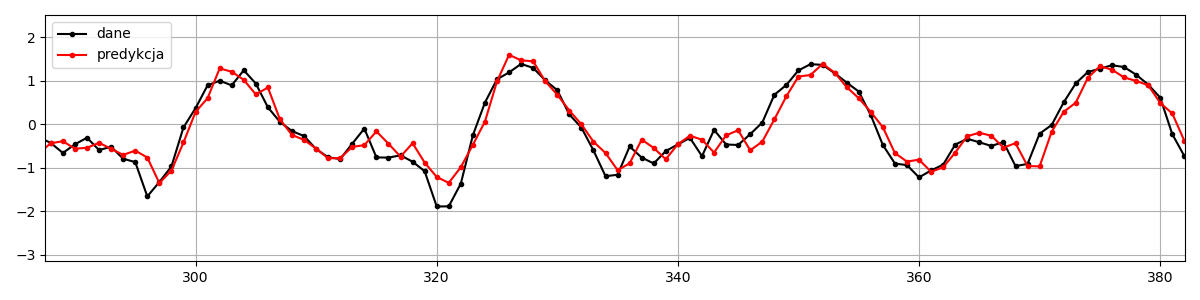
\includegraphics[width=\scaletwo\textwidth]{images/threehm_zoom.png}\end{center}
\end{frame}
\begin{frame}	\frametitle{10 pomiarów w historii i 3 neurony w w. ukrytej}
	\texttt{n\_window, layers = 10, [3]}
	\begin{center}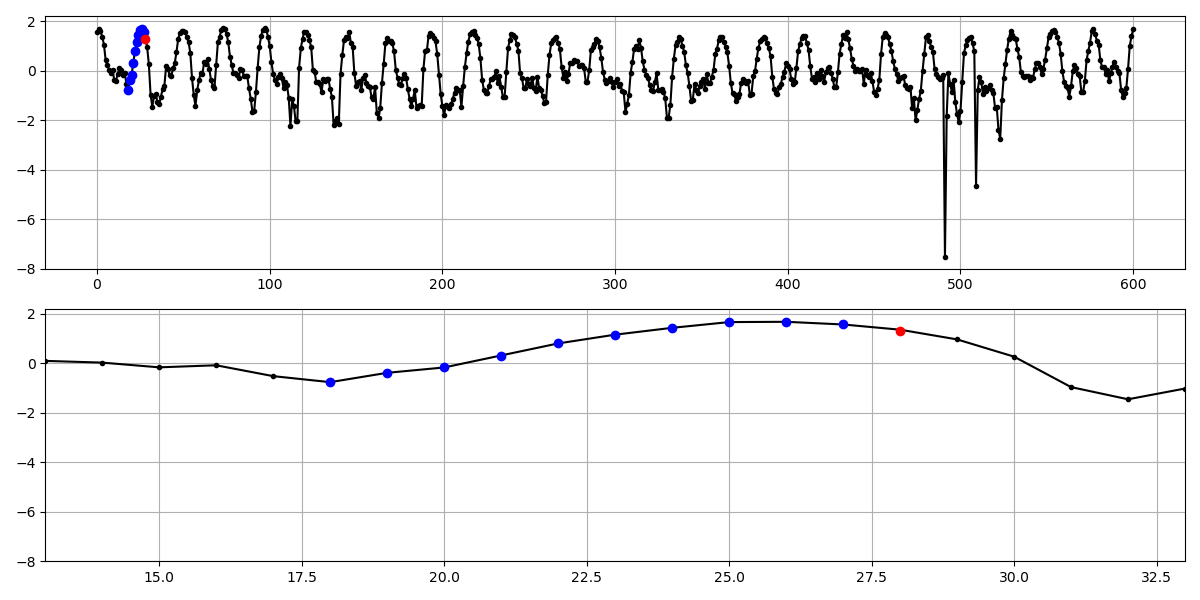
\includegraphics[width=\scaletwo\textwidth]{images/threehm_out.png}\end{center}
\end{frame}
\begin{frame}	\frametitle{10 pomiarów w historii i 3 neurony w w. ukrytej}
	\texttt{n\_window, layers = 10, [3]}
	\begin{center}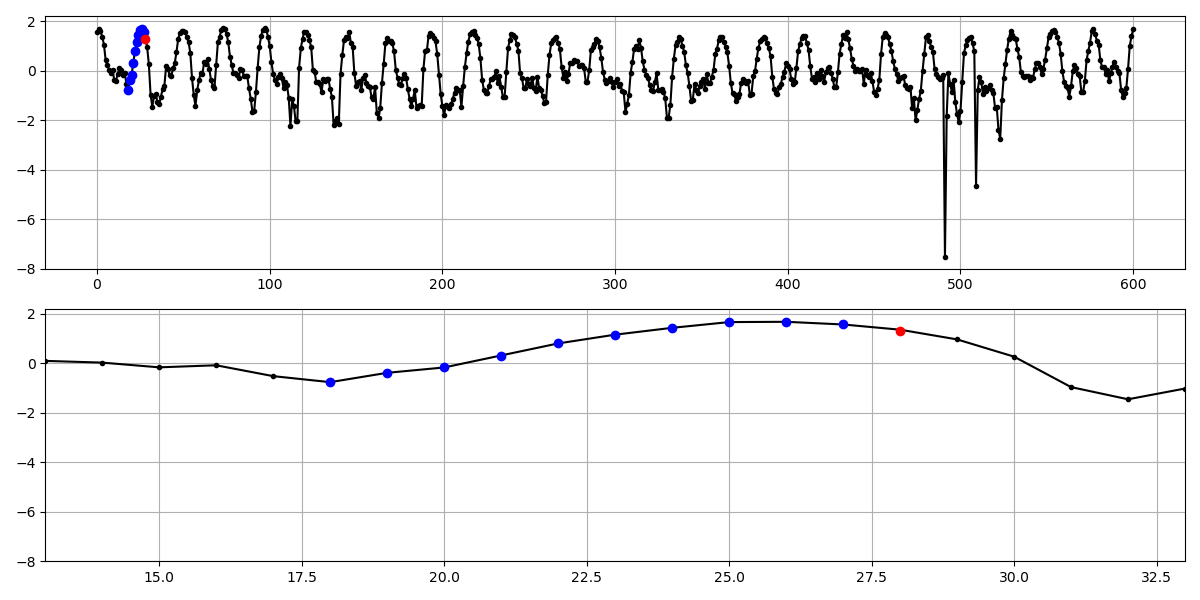
\includegraphics[width=0.49\textwidth]{images/threehm_out.png}
		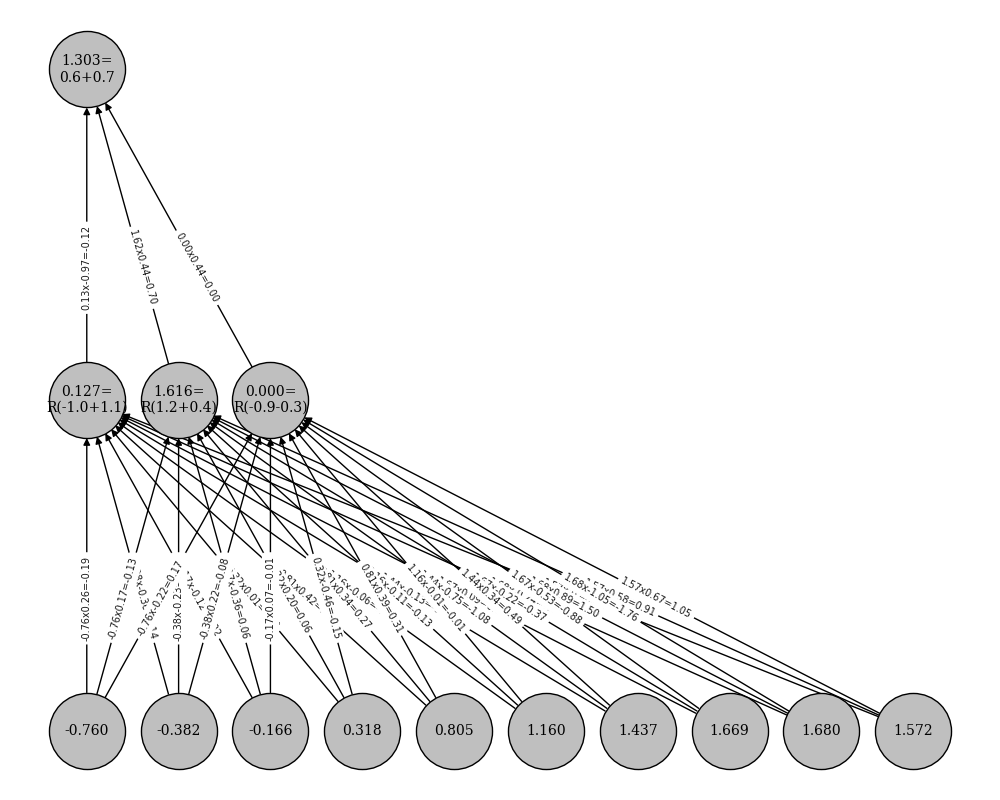
\includegraphics[width=0.49\textwidth]{images/threehm_in.png}\end{center}
\end{frame}

\begin{frame}	\frametitle{2 warstwy ukryte}
	\texttt{n\_window, layers = 10, [3, 2]}
	\begin{center}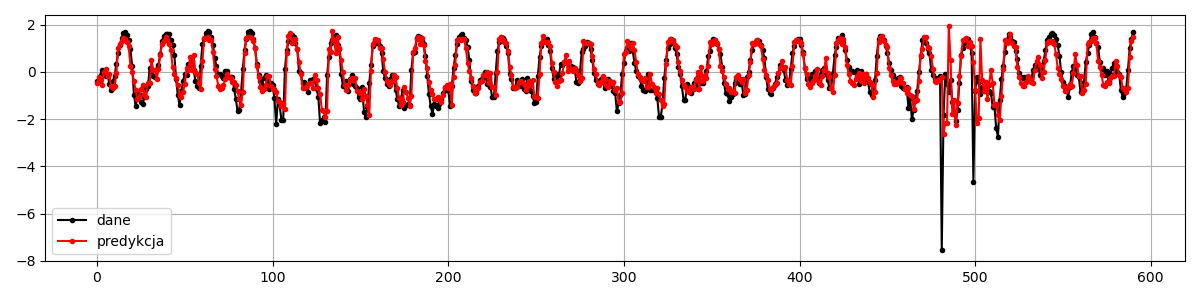
\includegraphics[width=\textwidth]{images/many_pred.png}\end{center}
\end{frame}
\begin{frame}	\frametitle{2 warstwy ukryte}
	\texttt{n\_window, layers = 10, [3, 2]}
	\begin{center}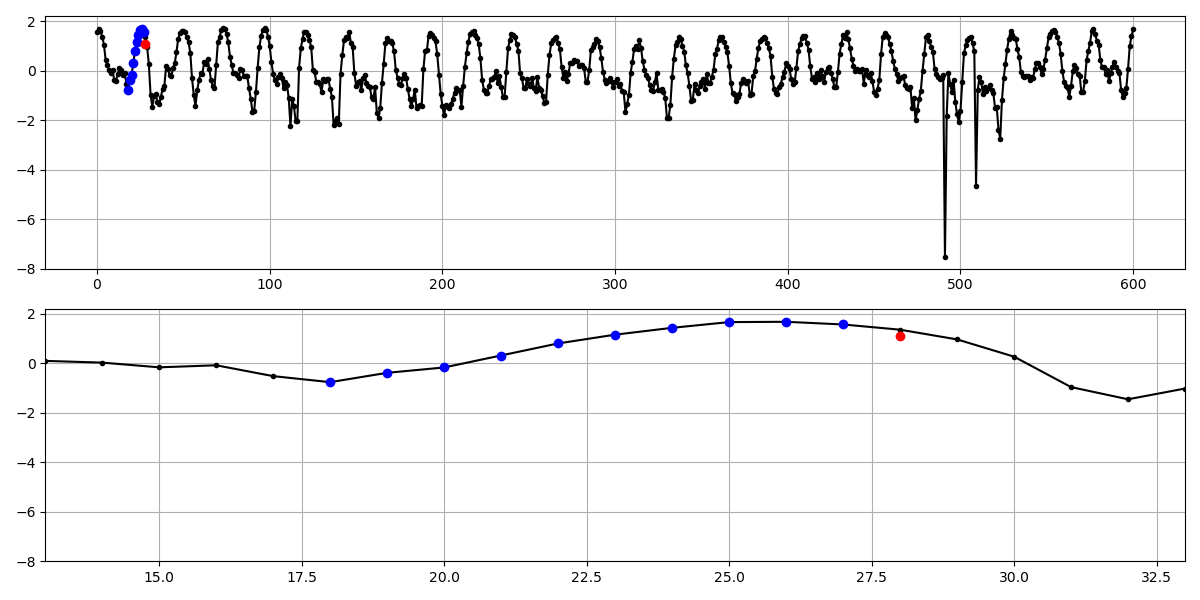
\includegraphics[width=\scaletwo\textwidth]{images/many_out.png}\end{center}
\end{frame}
\begin{frame}	\frametitle{2 warstwy ukryte}
	\texttt{n\_window, layers = 10, [3, 2]}
	\begin{center}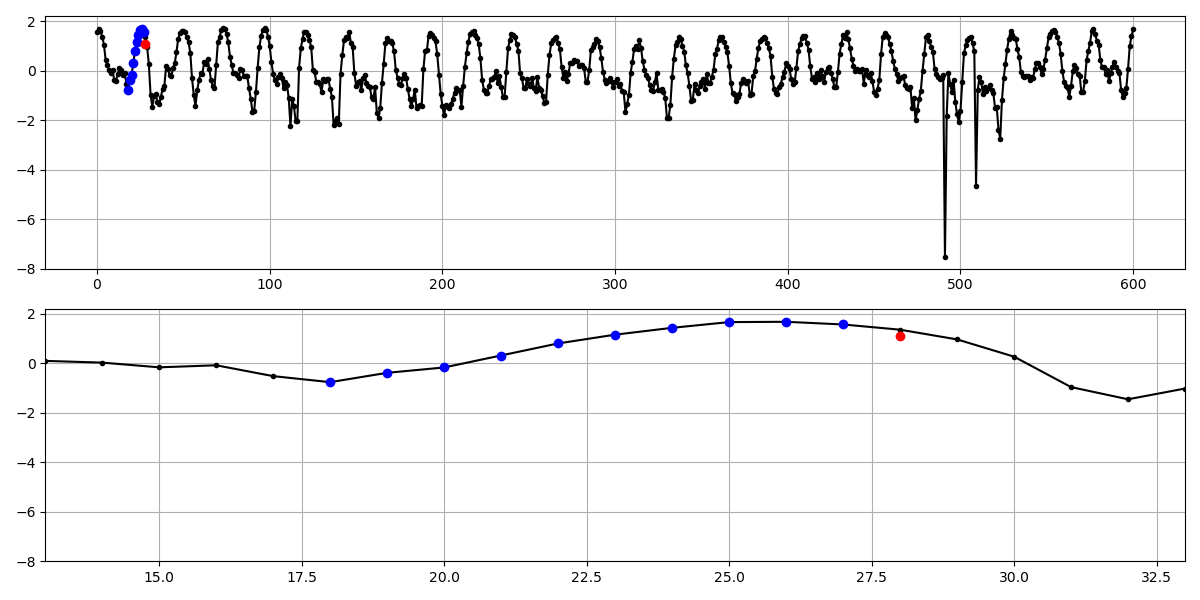
\includegraphics[width=0.49\textwidth]{images/many_out.png}
		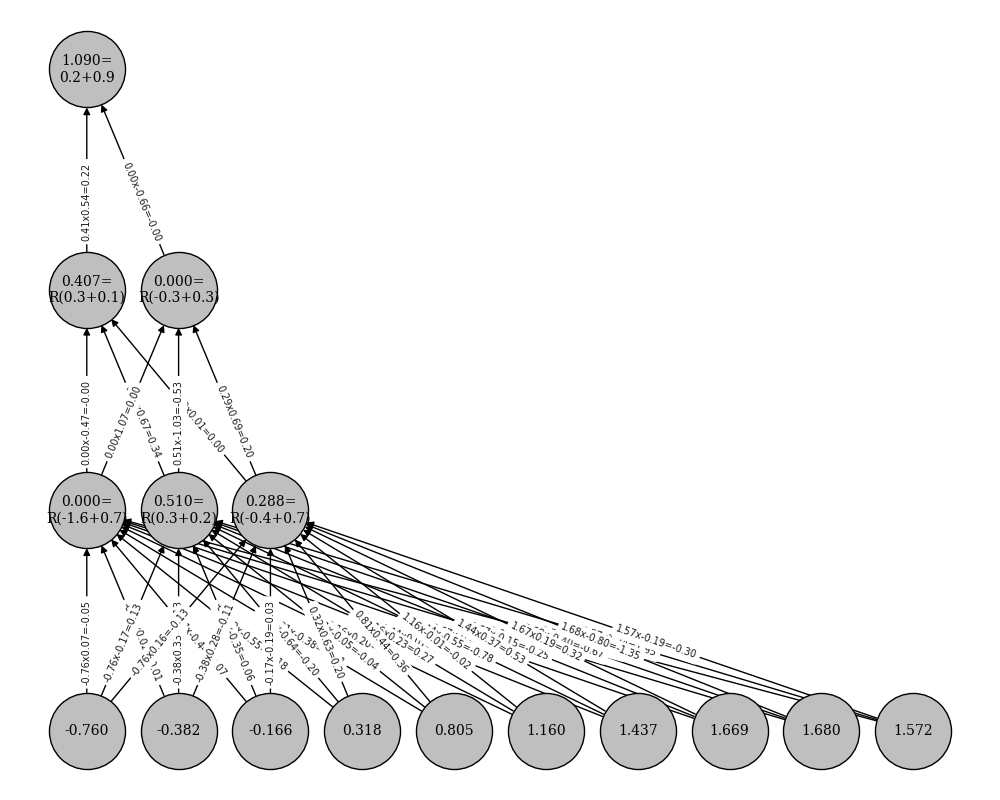
\includegraphics[width=0.49\textwidth]{images/many_in.png}\end{center}
\end{frame}

%\begin{frame}
%	\texttt{ex\_nn\_train.py}
%\end{frame}

\begin{frame}
	\frametitle{Wpływ wartości początkowych (10, [2])}
	\begin{center}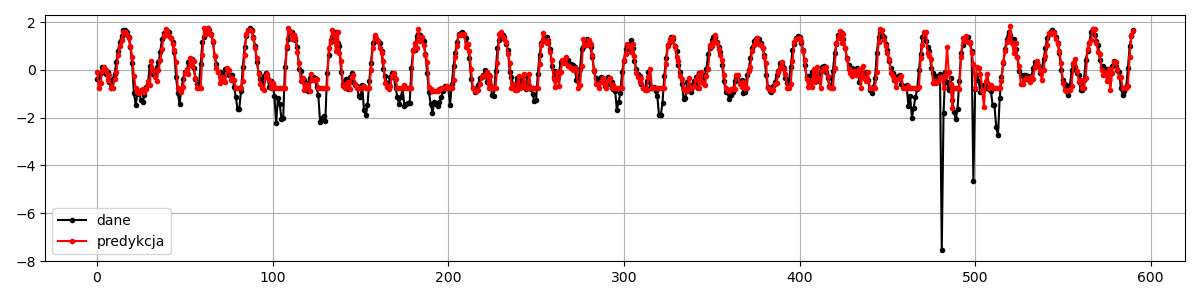
\includegraphics[width=\scalethree\textwidth]{images/rnd21.png}\end{center}
	\begin{center}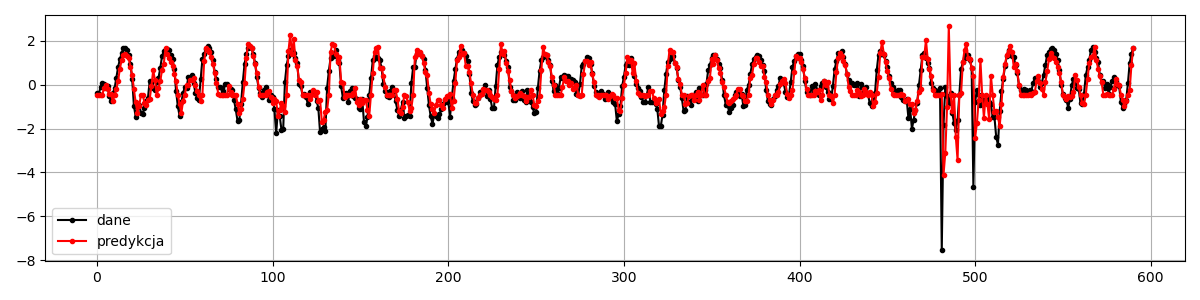
\includegraphics[width=\scalethree\textwidth]{images/rnd22.png}\end{center}
	\begin{center}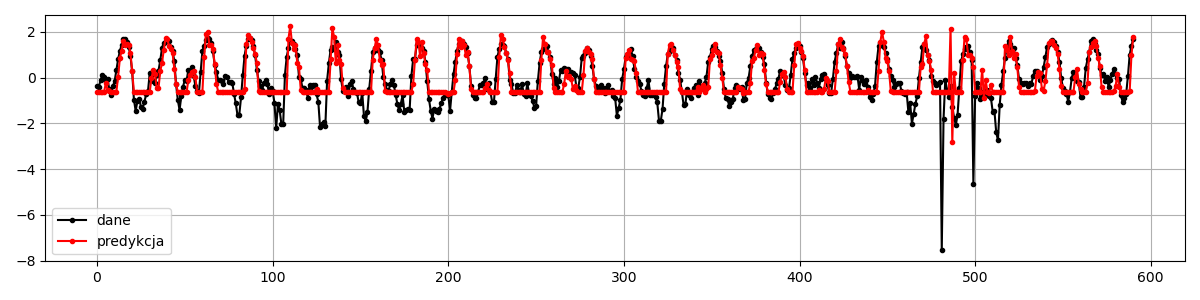
\includegraphics[width=\scalethree\textwidth]{images/rnd23.png}\end{center}
\end{frame}
\begin{frame}
	\frametitle{Wpływ wartości początkowych (1, [1])}
	\begin{center}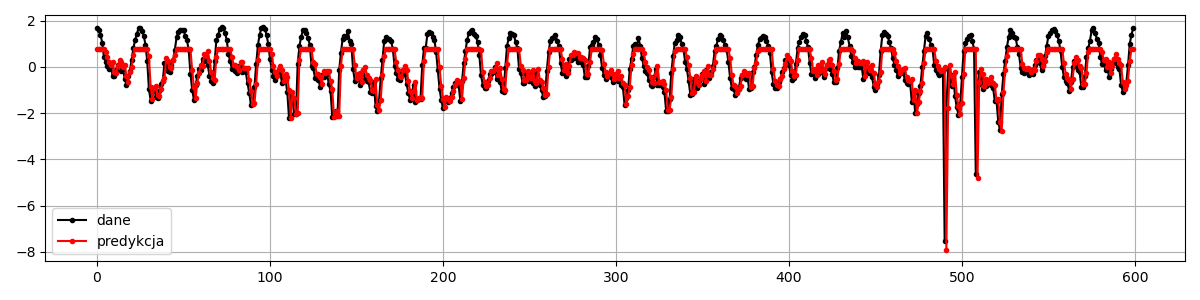
\includegraphics[width=\scalethree\textwidth]{images/rnd11.png}\end{center}
	\begin{center}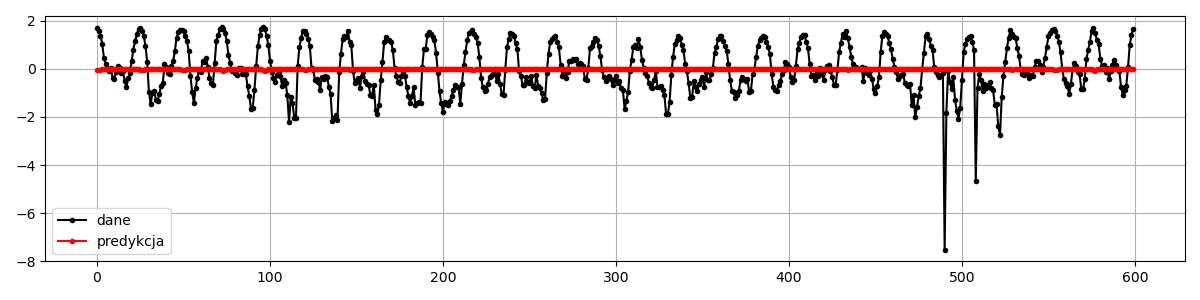
\includegraphics[width=\scalethree\textwidth]{images/rnd12.png}\end{center}
	\begin{center}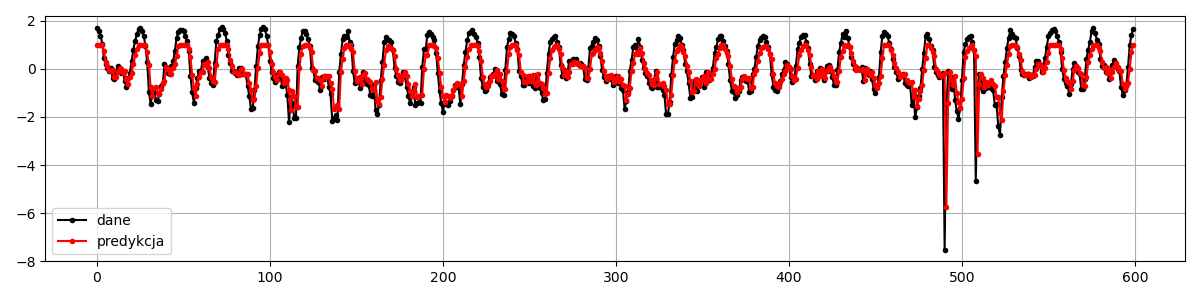
\includegraphics[width=\scalethree\textwidth]{images/rnd13.png}\end{center}
\end{frame}
\begin{frame}
	\frametitle{Wpływ liczby iteracji: 1, 10, 100}
	\begin{center}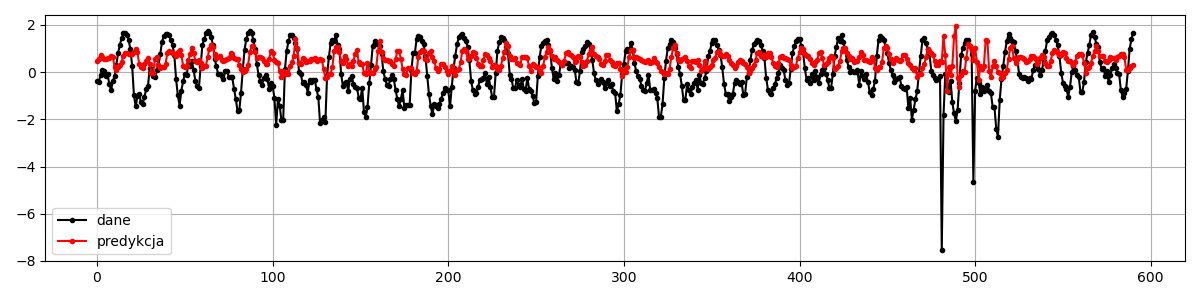
\includegraphics[width=\scalethree\textwidth]{images/loss1.png}\end{center}
	\begin{center}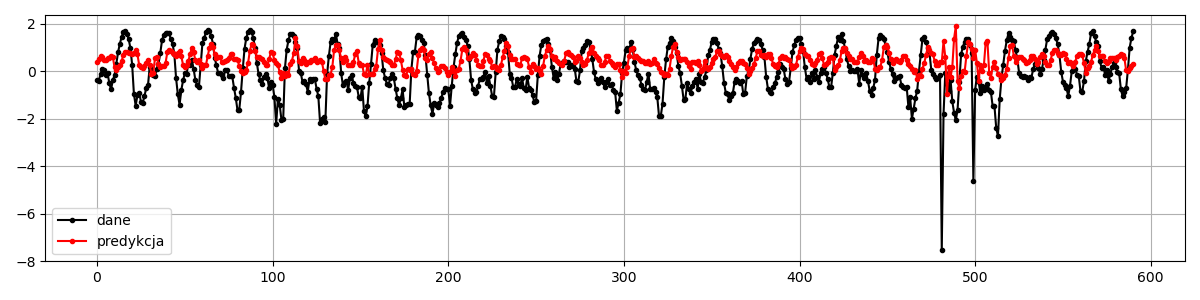
\includegraphics[width=\scalethree\textwidth]{images/loss10.png}\end{center}
	\begin{center}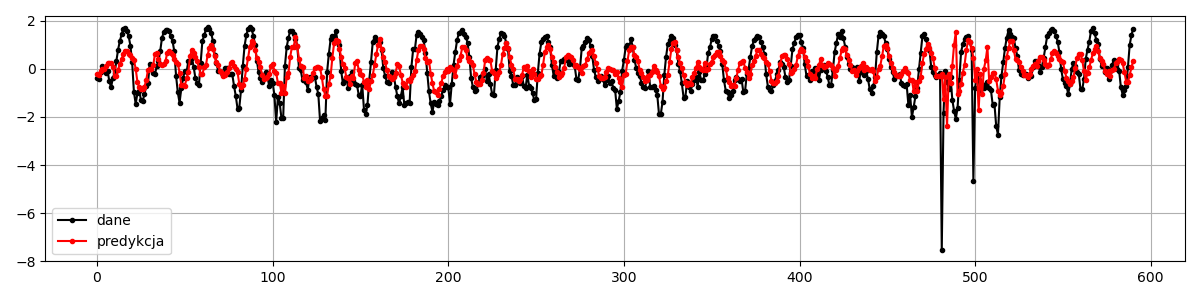
\includegraphics[width=\scalethree\textwidth]{images/loss100.png}\end{center}
\end{frame}
\begin{frame}
	\frametitle{Wpływ liczby iteracji: 200, 1000, 10000}
	\begin{center}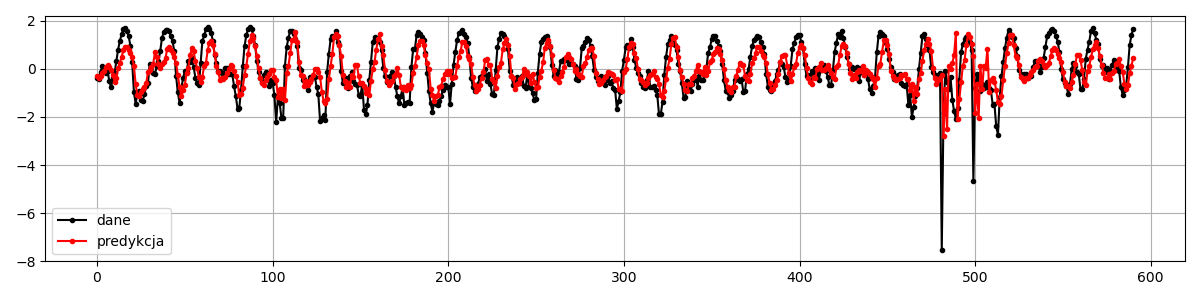
\includegraphics[width=\scalethree\textwidth]{images/loss200.png}\end{center}
	\begin{center}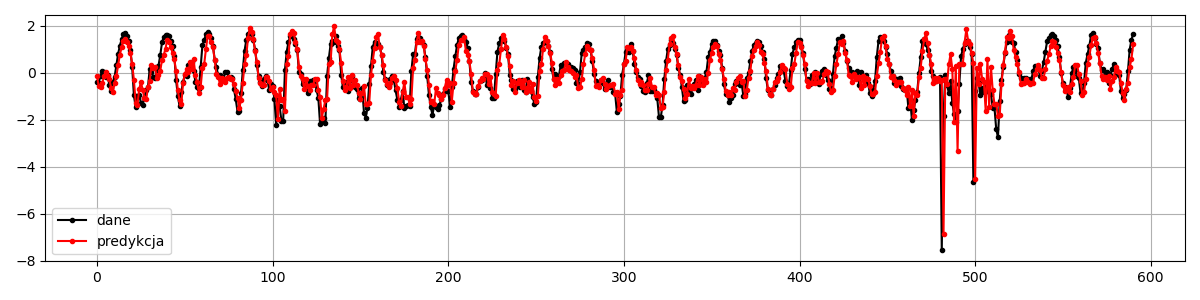
\includegraphics[width=\scalethree\textwidth]{images/loss1000.png}\end{center}
	\begin{center}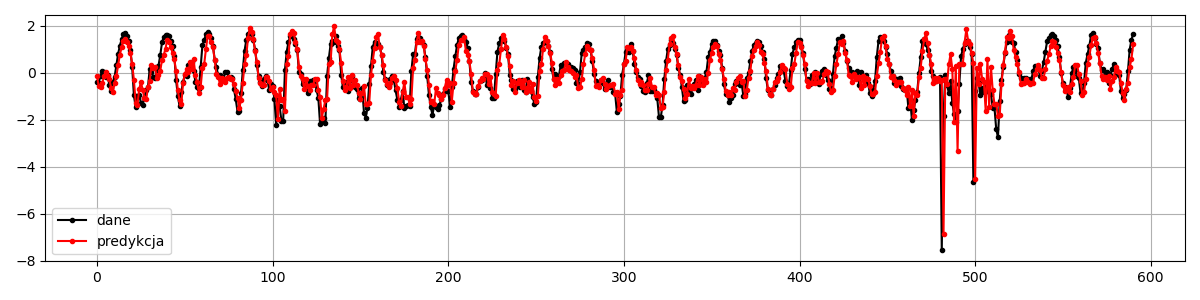
\includegraphics[width=\scalethree\textwidth]{images/loss10000.png}\end{center}
\end{frame}

\begin{frame}
	\frametitle{Inny sygnał?}
	\begin{center}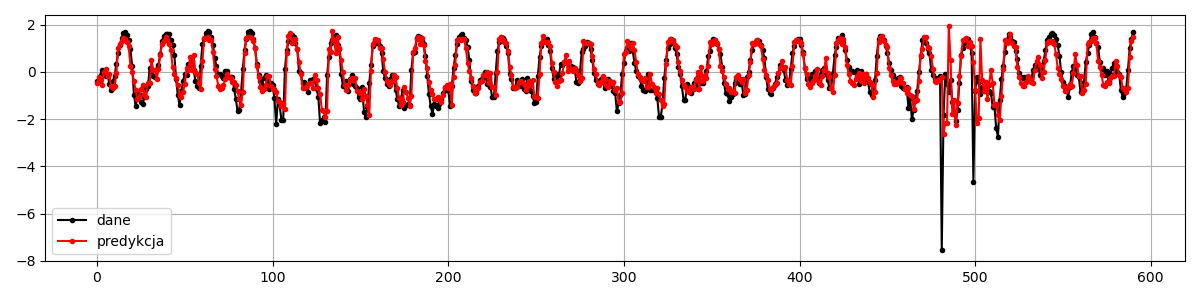
\includegraphics[width=\scalethree\textwidth]{images/cross1.png}\end{center}
	\begin{center}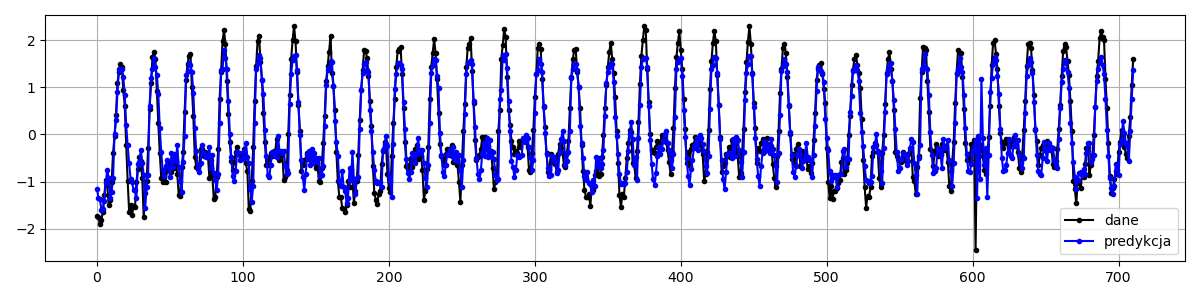
\includegraphics[width=\scalethree\textwidth]{images/cross2.png}\end{center}
	\begin{center}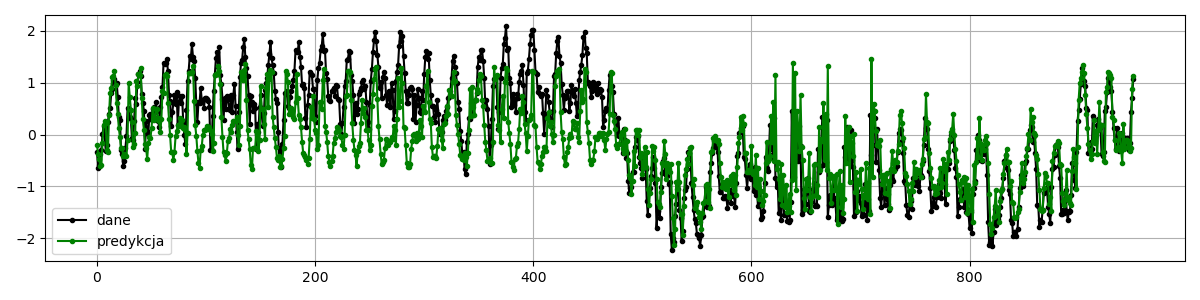
\includegraphics[width=\scalethree\textwidth]{images/cross3.png}\end{center}
\end{frame}

%
%\begin{frame}
%	\frametitle{Podsumowanie -- zastosowanie sieci neuronowych}
%	\begin{enumerate}
%		\item Możliwości odwzorowania wzorców
%		\item Zbiór/zbiory danych (reprezentatywność!)
%		\item Dobór hiperparametrów (np. liczba neuronów)
%		\item Zbiory treningowe, testowe, walidacyjne
%		\item Wpływ losowości (stan początkowy)
%		\item Problemy z douczaniem
%		\item Czas obliczeń (głównie trening), wymagana pamięć
%		\item Model ,,czarno-skrzynkowy''
%	\end{enumerate}
%\end{frame}
%
%\begin{frame}
%	\frametitle{Podsumowanie -- złożoność sieci neuronowych}
%	\begin{enumerate}
%		\item Zaprezentowana
%			\begin{description}
%				\item[liczba parametrów] 25 (10, [2])
%				\item[czas trenowania] sekundy
%			\end{description}
%		\item ChatGPT GPT-4 (prawdopodobnie)
%			\begin{description}
%				\item[liczba parametrów] 1,76 biliona 
%				\item[czas trenowania] trzy miesiące na 25,000 Nvidia A100 GPU (ponad 3 tys. serwerów)
%			\end{description}
%		
%	\end{enumerate}
%\end{frame}

\begin{frame}
	\frametitle{Podsumowanie -- wykrywanie anomalii}
	\begin{center}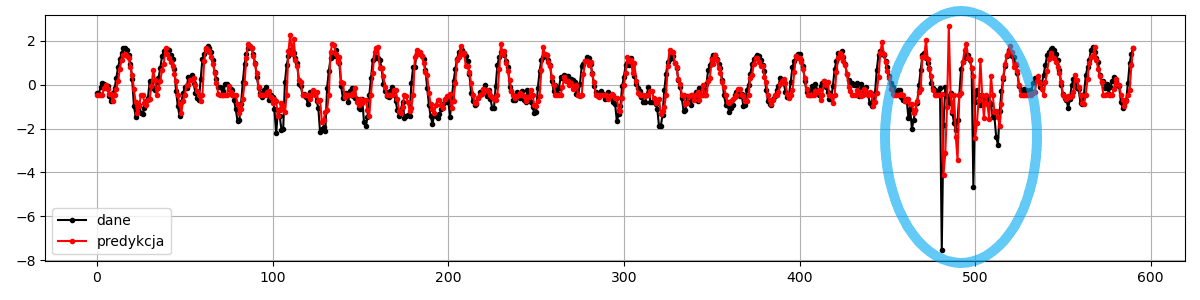
\includegraphics[width=\textwidth]{images/appl.png}\end{center}
\end{frame}

%\begin{frame}
%	\frametitle{Podsumowanie -- możliwości sieci neuronowych}
%	\begin{enumerate}
%		\item Klasyfikacja -- rozpoznawanie 
%		\item Predykcja -- generowanie sygnałów
%	\end{enumerate}
%\end{frame}
%
%
%\begin{frame}
%	\frametitle{Sieci neuronowe a algorytmy statystyczne}
%	\begin{center}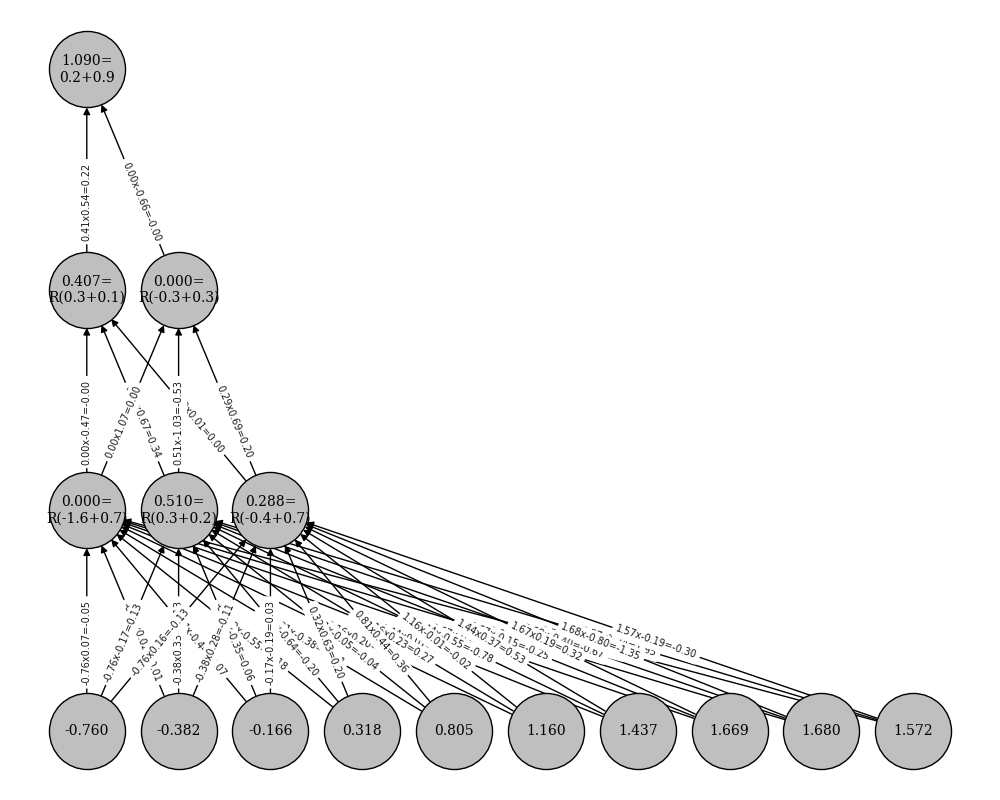
\includegraphics[width=0.49\textwidth]{images/many_in.png}
%		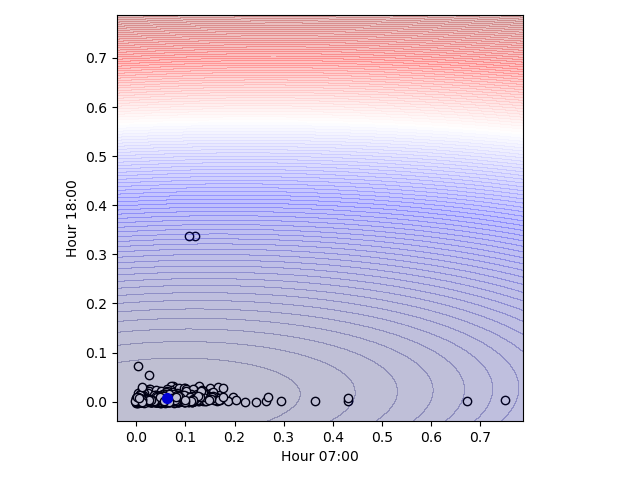
\includegraphics[width=0.49\textwidth]{images/C.png}\end{center}
%\end{frame}
%
%
%
%\section{Systemy baz danych przestrzennych}
%
%
%\begin{frame}
%	\frametitle{Bazy danych przestrzennych -- sieć dystrybucji wody}
%%	\begin{enumerate}
%%		\item Przechowywanie 
%%		\item Weryfikacja
%%	\end{enumerate}
%\begin{center}\includegraphics[width=1\textwidth]{images/KotaKinabalu_Sabah_Public-Water-Supply-01.jpg}\end{center}
%{\tiny https://commons.wikimedia.org/wiki/File:KotaKinabalu\_Sabah\_Public-Water-Supply-01.jpg, Photo by CEphoto, Uwe Aranas}
%\end{frame}
%
%\begin{frame}
%	\frametitle{Bazy danych przestrzennych -- QGIS}
%	%	\begin{enumerate}
%	%		\item Przechowywanie 
%	%		\item Weryfikacja
%	%	\end{enumerate}
%	\begin{center}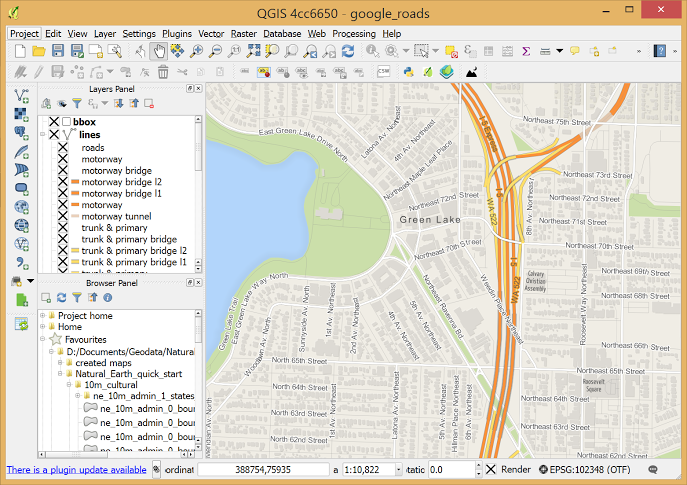
\includegraphics[width=1\textwidth]{images/qgis.png}\end{center}
%	{\tiny źródło: QGIS}
%\end{frame}
%\begin{frame}
%	\frametitle{Bazy danych przestrzennych -- QGIS}
%	%	\begin{enumerate}
%	%		\item Przechowywanie 
%	%		\item Weryfikacja
%	%	\end{enumerate}
%	\begin{center}
\includegraphics[width=1\textwidth]{images/qgist.png}\end{center}
%	{\tiny źródło: QGIS}
%\end{frame}
%
%\begin{frame}
%	\frametitle{Model hydrauliczny sieci dystrybucji wody}
%	%	\begin{enumerate}
%	%		\item Przechowywanie 
%	%		\item Weryfikacja
%	%	\end{enumerate}
%	\begin{center}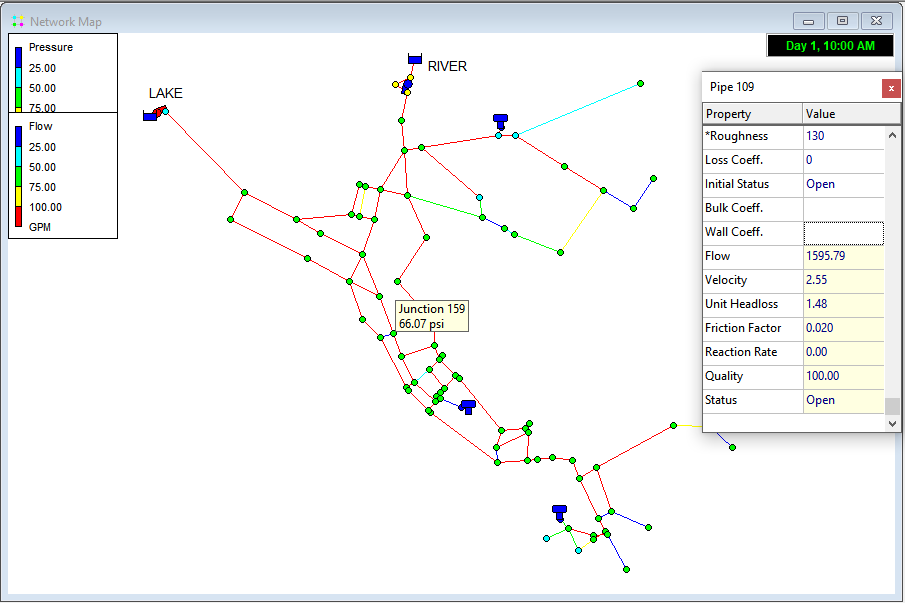
\includegraphics[width=1\textwidth]{images/hydraulic.png}\end{center}
%\end{frame}
%
%\begin{frame}
%	\frametitle{Przygotowywanie modelu hydraulicznego}
%	\begin{enumerate}
%		\item Dane GIS (ang. Geographic Information System) sieci $\rightarrow$ QGIS
%		\item Korekta danych
%		\item Pobranie danych (zużycie, ciśnienia)
%		\item Budowa modelu  $\rightarrow$ EPANET
%		\item Weryfikacja, kalibracja
%		\item Wykorzystanie modelu -- np. lokalizacja prawdopodobnych obszarów wycieków
%	\end{enumerate}
%\end{frame}
%
%\begin{frame}
%	\frametitle{EPANET}
%	\url{https://www.epa.gov/water-research/epanet}
%\end{frame}
%


\end{document}

